\documentclass[12pt,onecolumn]{article}
\usepackage[utf8]{inputenc} % UTF8 input encoding
\usepackage[T2A]{fontenc}   % T2A font encoding for Cyrillic script
\usepackage[russian]{babel} % Russian language support
\usepackage{listings}
\usepackage{float}
\usepackage{mathtools}
\everymath{\displaystyle}
\usepackage{listings} 
\usepackage[usenames]{color}
\usepackage{geometry}
\usepackage{verbatim}
\usepackage{tabularray}
\usepackage{color}
\usepackage{hyperref}
\newcommand{\nparagraph}[1]{\paragraph{#1}\mbox{}\\}
\geometry{
  a4paper,
  top=20mm, 
  right=25mm, 
  bottom=20mm, 
  left=20mm
}

\begin{document}
\setcounter{tocdepth}{4}
\begin{center}
    Федеральное государственное автономное образовательное учреждение высшего образования "Национальный Исследовательский Университет ИТМО"\\ 
    Мегафакультет Компьютерных Технологий и Управления\\
    Факультет Программной Инженерии и Компьютерной Техники \\
    
\includegraphics[scale=0.3]{image/itmo.jpg} % нужно закинуть картинку логтипа в папку с отчетом
\end{center}
\vspace{1cm}


\begin{center}
    \textbf{Лабораторная работа 2}\\
    \textit{"Локальные сети"}\\
    по дисциплине\\
    \textbf{Компьютерные сети}
\end{center}

\vspace{2cm}

\begin{flushright}
  Выполнил Студент  группы P33102\\
  \textbf{Лапин Алексей Александрович}\\
  Преподаватель: \\
  \textbf{Авксентьева Елена Юрьевна}\\
\end{flushright}

\vspace{6cm}
\begin{center}
    г. Санкт-Петербург\\
    2023г.
\end{center}

\newpage
\tableofcontents
\newpage

\section*{Цель работы}\addcontentsline{toc}{section}{Цель работы}
Изучение принципов настройки и функционирования локальных сетей, построенных с использованием концентраторов и коммутаторов, а также процессов передачи данных на основе стека протоколов TCP/IP, с использованием программы моделирования компьютерных сетей NetEmul.

В процессе выполнения лабораторной работы (ЛР) необходимо:

\begin{enumerate}
    \item построить три модели локальной сети: с использованием концентратора, коммутатора и многосегментную сеть;
    \item выполнить настройку сети, заключающуюся в присвоении IP-адре интерфейсам сети;
    \item выполнить тестирование разработанных сетей путем проведения экспериментов по передаче данных (пакетов и кадров) на основе протоколов UDP и TCP;
    \item проанализировать результаты тестирования и сформулировать выводы о б эффективности смоделированных вариантов построения локальных сетей;
    \item сохранить разработанные модели локальных сетей для демонстрации процессов передачи данных при защите лабораторной работы.
\end{enumerate}
\section*{Вариант}
Вариант 4

P33102 Лапин Алексей Александрович

Ф = 5, И = 7, О = 13, Н = 2

Исходный адрес: $(7 + 2 + 128).(13+2).(5+2).(5+7) = 137.15.7.12 ... 137.15.7.21$

$N_1 = 2; N_2 = 3; N_3 = 3$

\section{Локальная сеть с концентратором (Сеть 1)}
\subsection{Построение сети с концентратором.}
\begin{figure}[H]
    \centering
    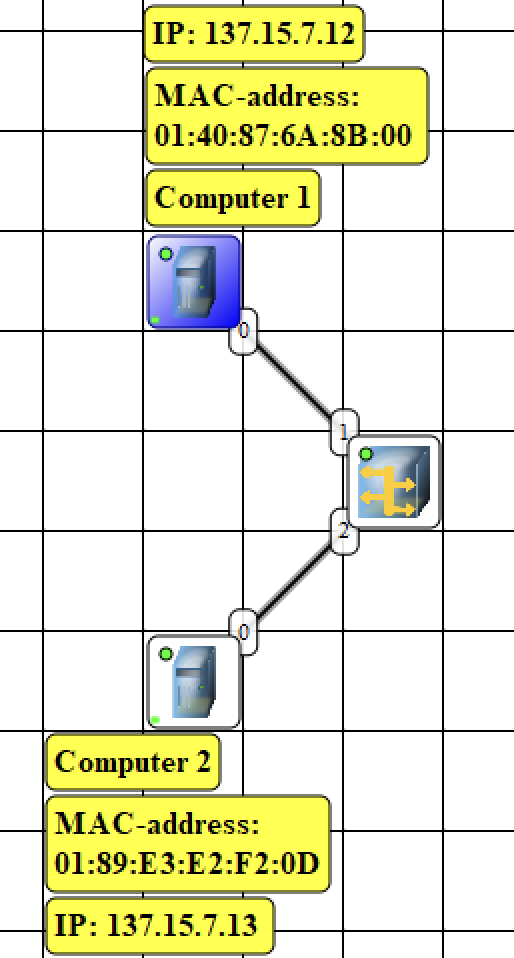
\includegraphics[scale=0.5]{image/part1/topology.png}
    \caption{Схема сети из двух компьютеров с концентратором}
\end{figure}
Таблицы маршрутизации компьютеров, до назначения IP-адресов:
\begin{figure}[H]
    \centering
    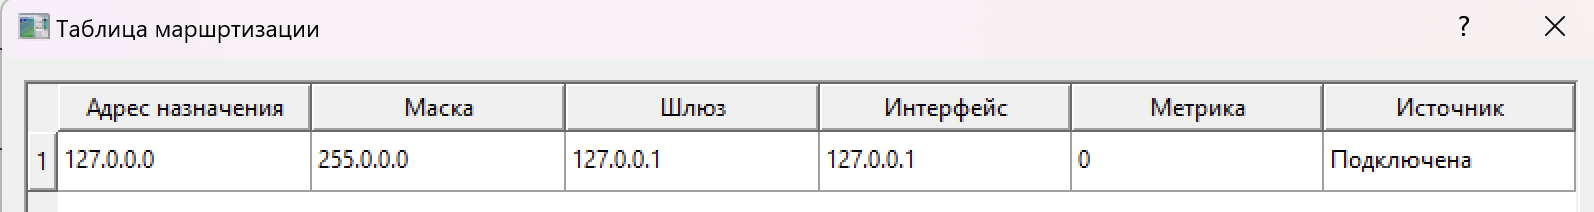
\includegraphics[scale=0.5]{image/part1/routing-table-1.png}
    \caption{Таблица маршрутизации компьютера 1}
\end{figure}
Адреса 127.0.0.0 и 127.0.0.1 - это системные адреса, которые используются для обратной петли (loopback) в локальной сети.
\begin{figure}[H]
    \centering
    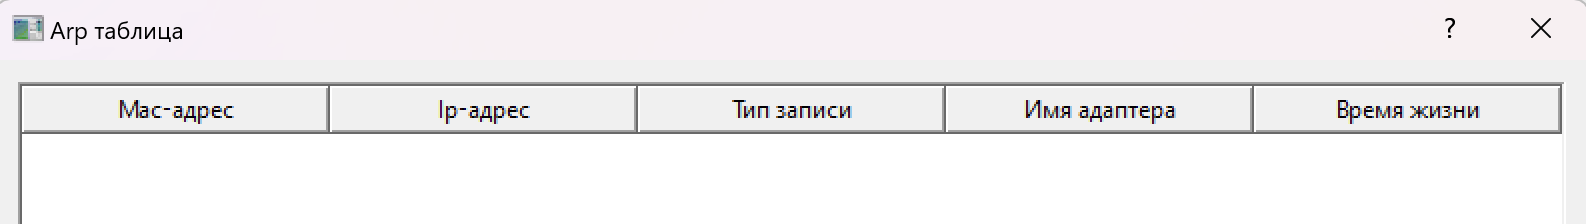
\includegraphics[scale=0.5]{image/part1/arp-table.png}
    \caption{Таблица ARP}
\end{figure}
ARP-таблицы на компьютерах пока что пусты.
Так как для ее заполнения необходимо знать
IP адреса. Когда знает, то посылается широковещательный ARP-запрос для поиска нужного устройства.
Устройство с нужным IP-адресом отвечает на запрос и его MAC-адрес добавляется в ARP-таблицу.
На данном этапе ARP запросы еще не были посланы.
\subsection{Настройка компьютеров.}
В процессе настройки компьютеров были присвоены IP-адреса: 137.15.7.12 и 137.15.7.13 для Компьютера 1 и Компьютера 2 соответственно.
Маска подсети была присвоена автоматически.
При добавлении IP-адреса, каждый компьютер отправляет широковещательный ARP-запрос следующего вида:
\begin{figure}[H]
    \centering
    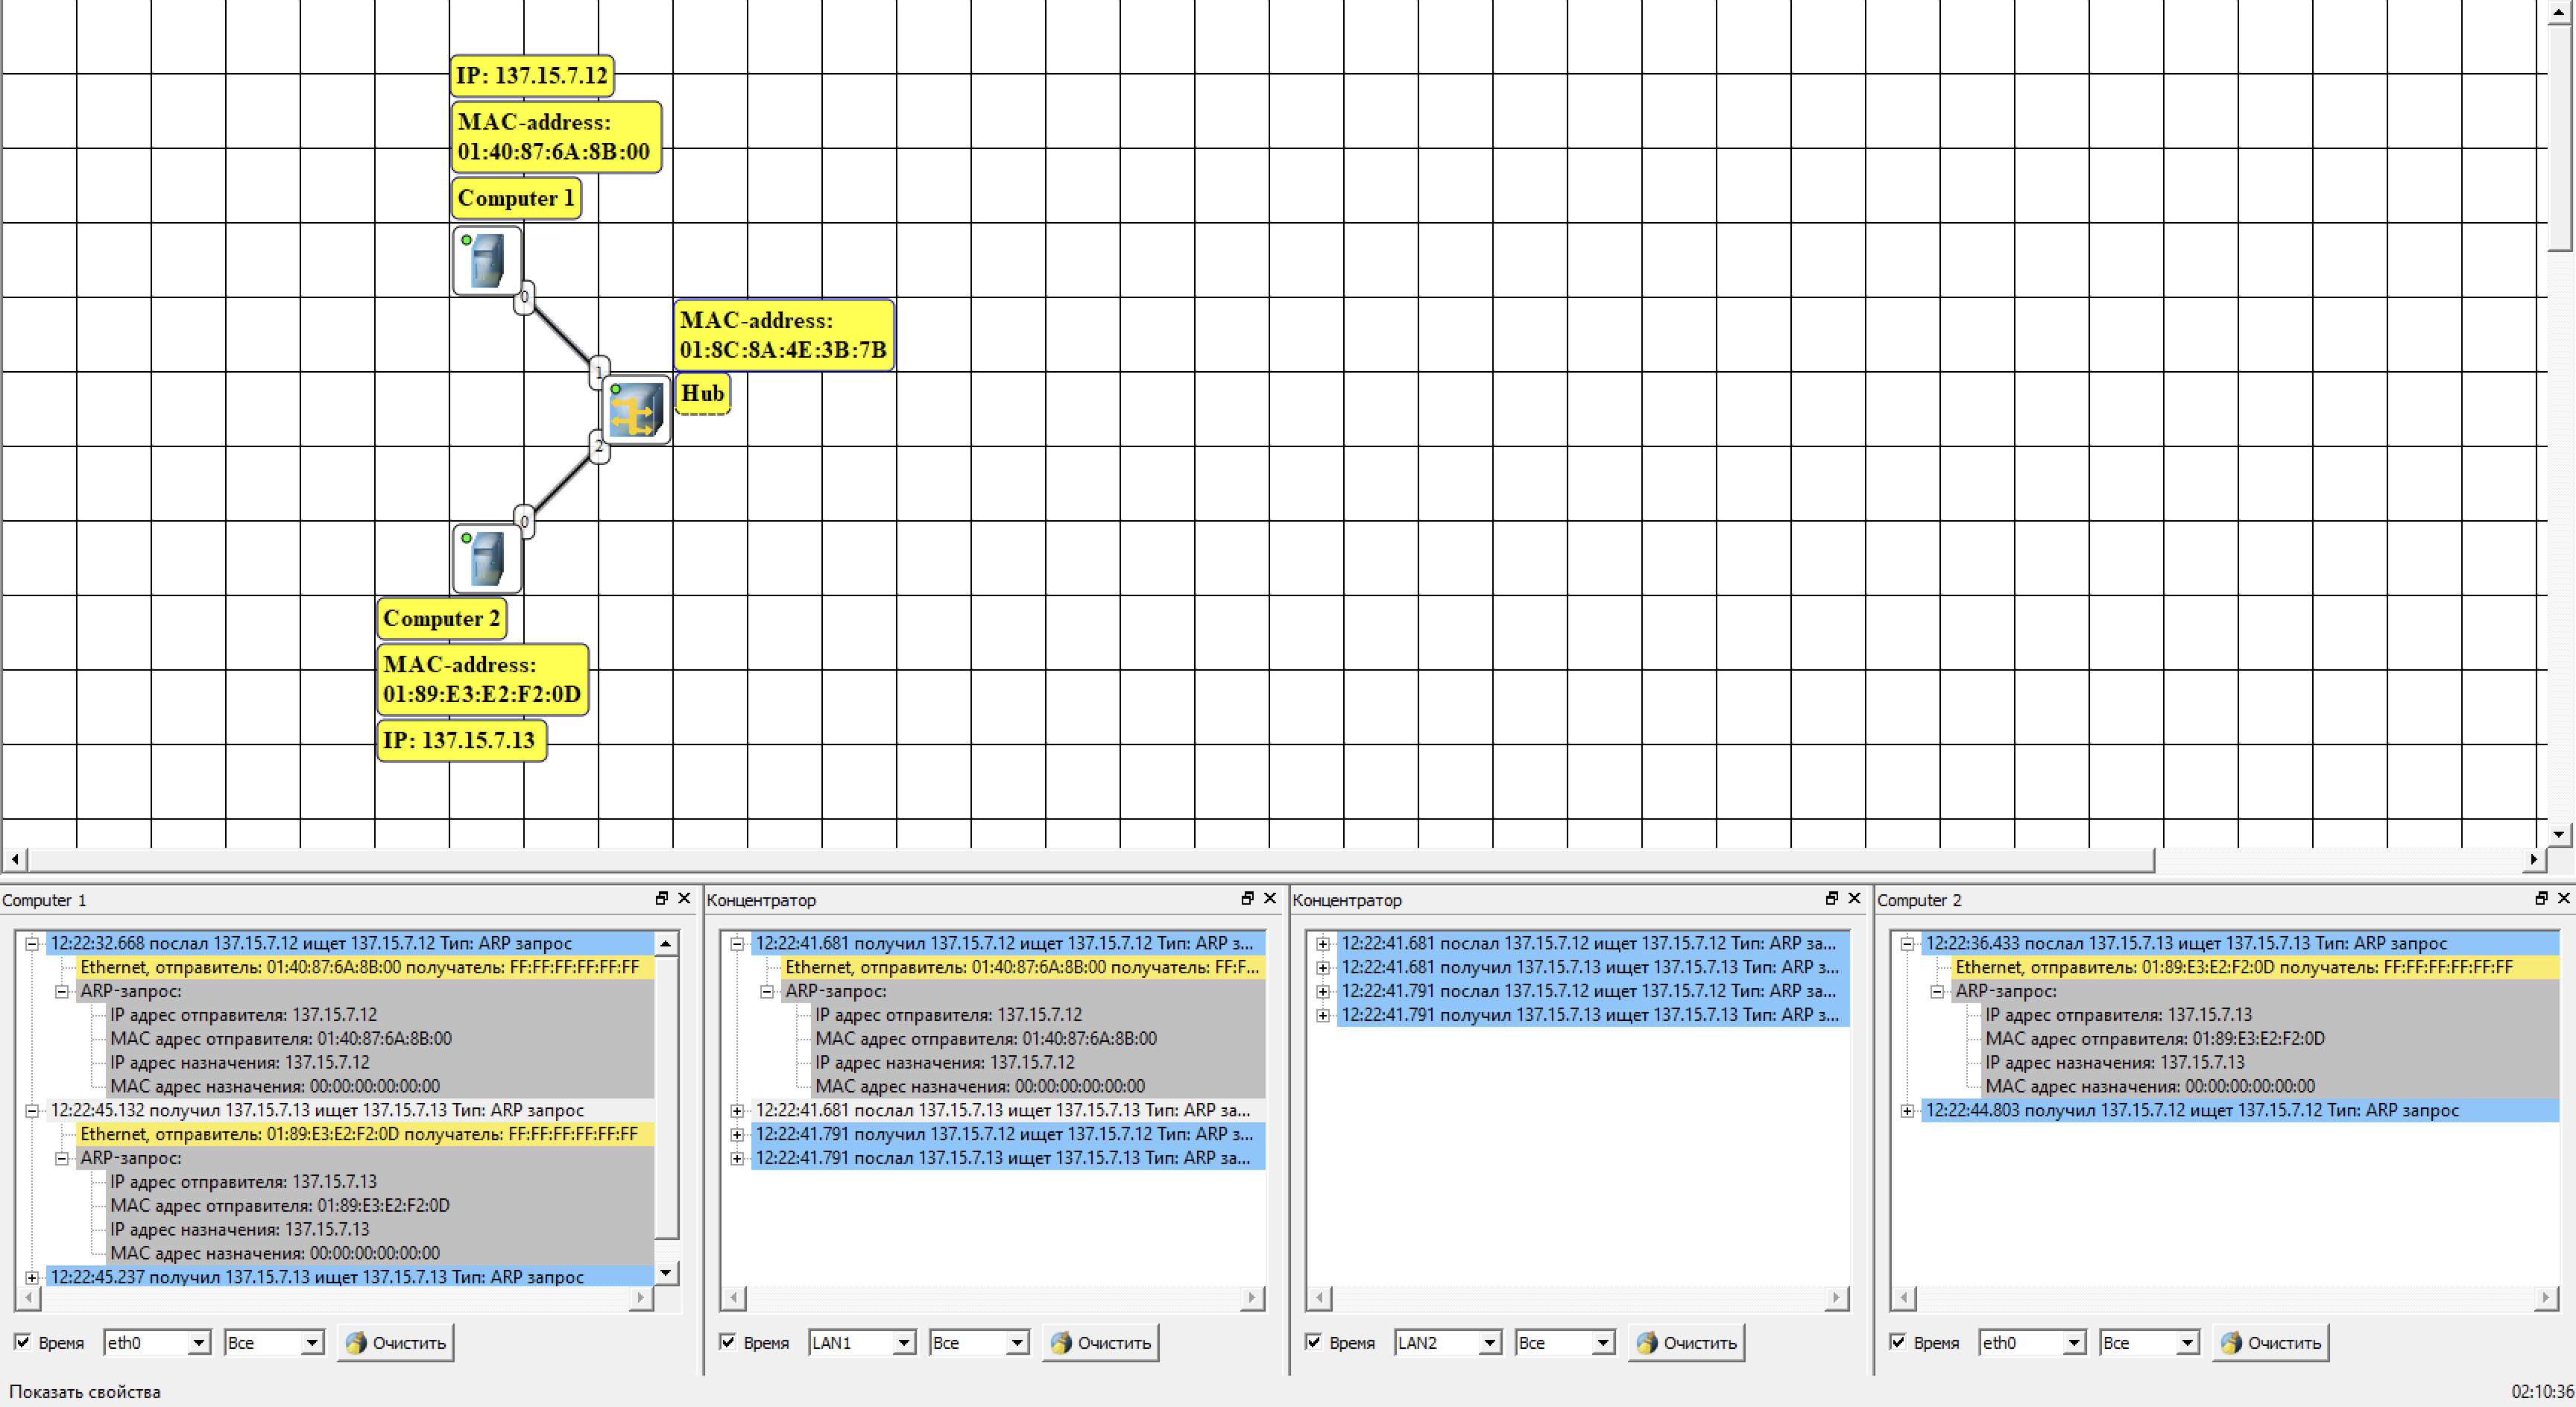
\includegraphics[width=\textwidth]{image/part1/arp-request1.png}
    \caption{Настройка IP-адресов}
\end{figure}

С помощью этого ARP-запроса компьютер хочет удостовериться, что в данной сети ещё нет устройства с таким же IP-адресом.

Каждый из подключенных компьютеров получает этот ARP-запрос, но поскольку никто из них не имеет такого же адреса – ответ отправлен не будет.

\subsection{Анализ таблиц.}
\begin{figure}[H]
  \centering
  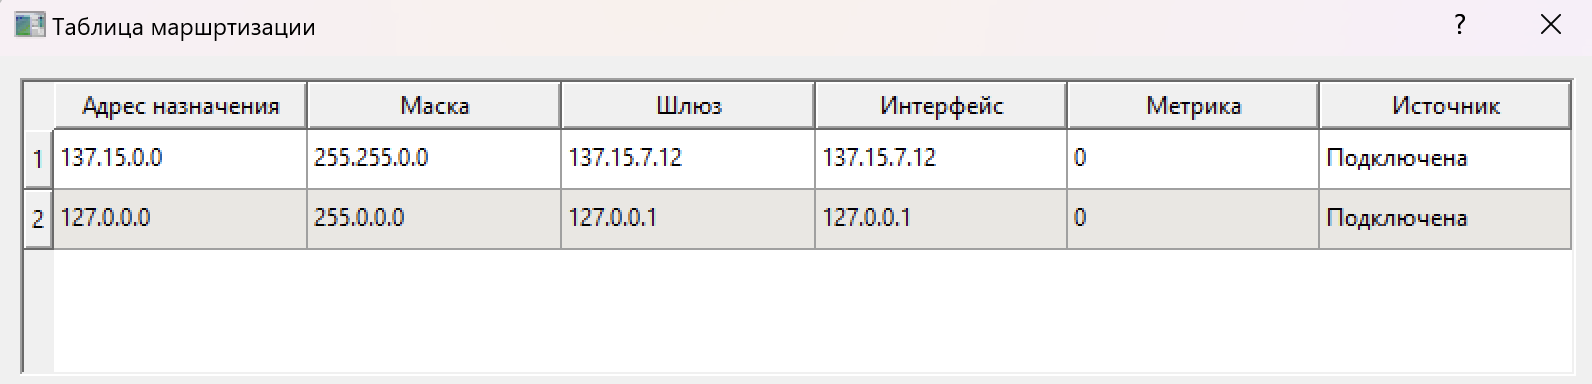
\includegraphics[width=\textwidth]{image/part1/route-table-1.png}
  \caption{Таблица маршрутизации компьютера 1}
\end{figure}
\begin{figure}[H]
  \centering
  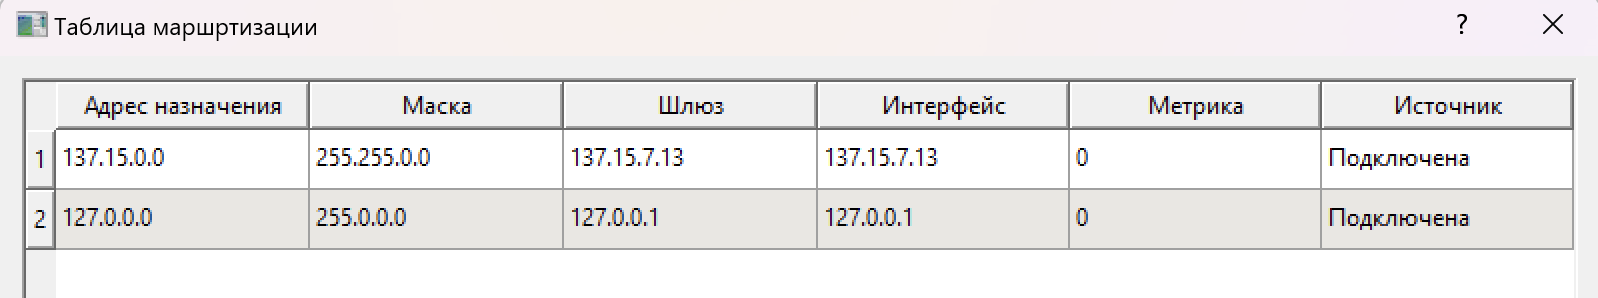
\includegraphics[width=\textwidth]{image/part1/route-table-2.png}
  \caption{Таблица маршрутизации компьютера 2}
\end{figure}
В каждый компьютер добавилась ещё одна запись, описывающая шлюз локальной сети, в которой находится компьютер.

ARP-таблицы перестали быть пустыми:
\begin{figure}[H]
  \centering
  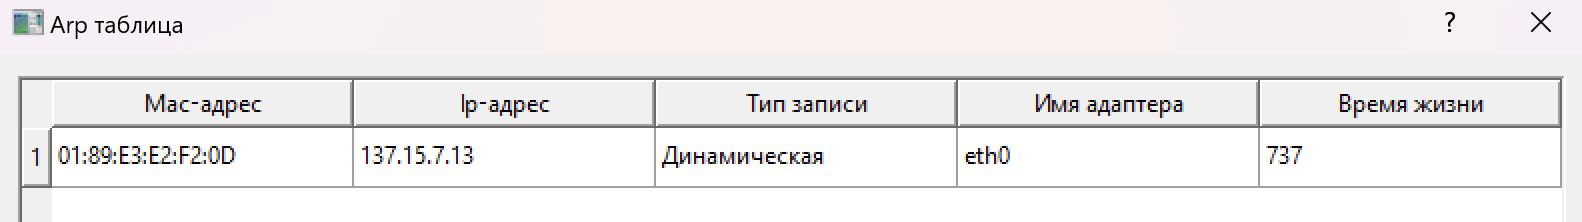
\includegraphics[width=\textwidth]{image/part1/arp-table-1.png}
  \caption{Таблица ARP компьютера 1}
\end{figure}
\begin{figure}[H]
  \centering
  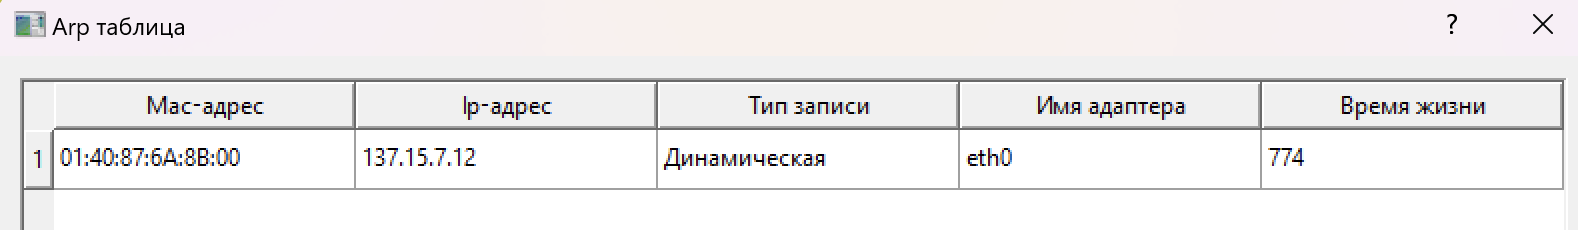
\includegraphics[width=\textwidth]{image/part1/arp-table-2.png}
  \caption{Таблица ARP компьютера 2}
\end{figure}
Теперь в них содержатся связки MAC-IP своих «соседей» по сети.

"Время жизни" означает, что если компьютер по какой-либо причине не смог отправить запрос на изменение или удаление записи из ARP-таблицы других компьютеров, запись все равно будет удалена через определенное количество времени.

\subsection{Тестирование сети (отправка пакетов).}
\subsubsection{UDP}
\begin{figure}[H]
  \centering
  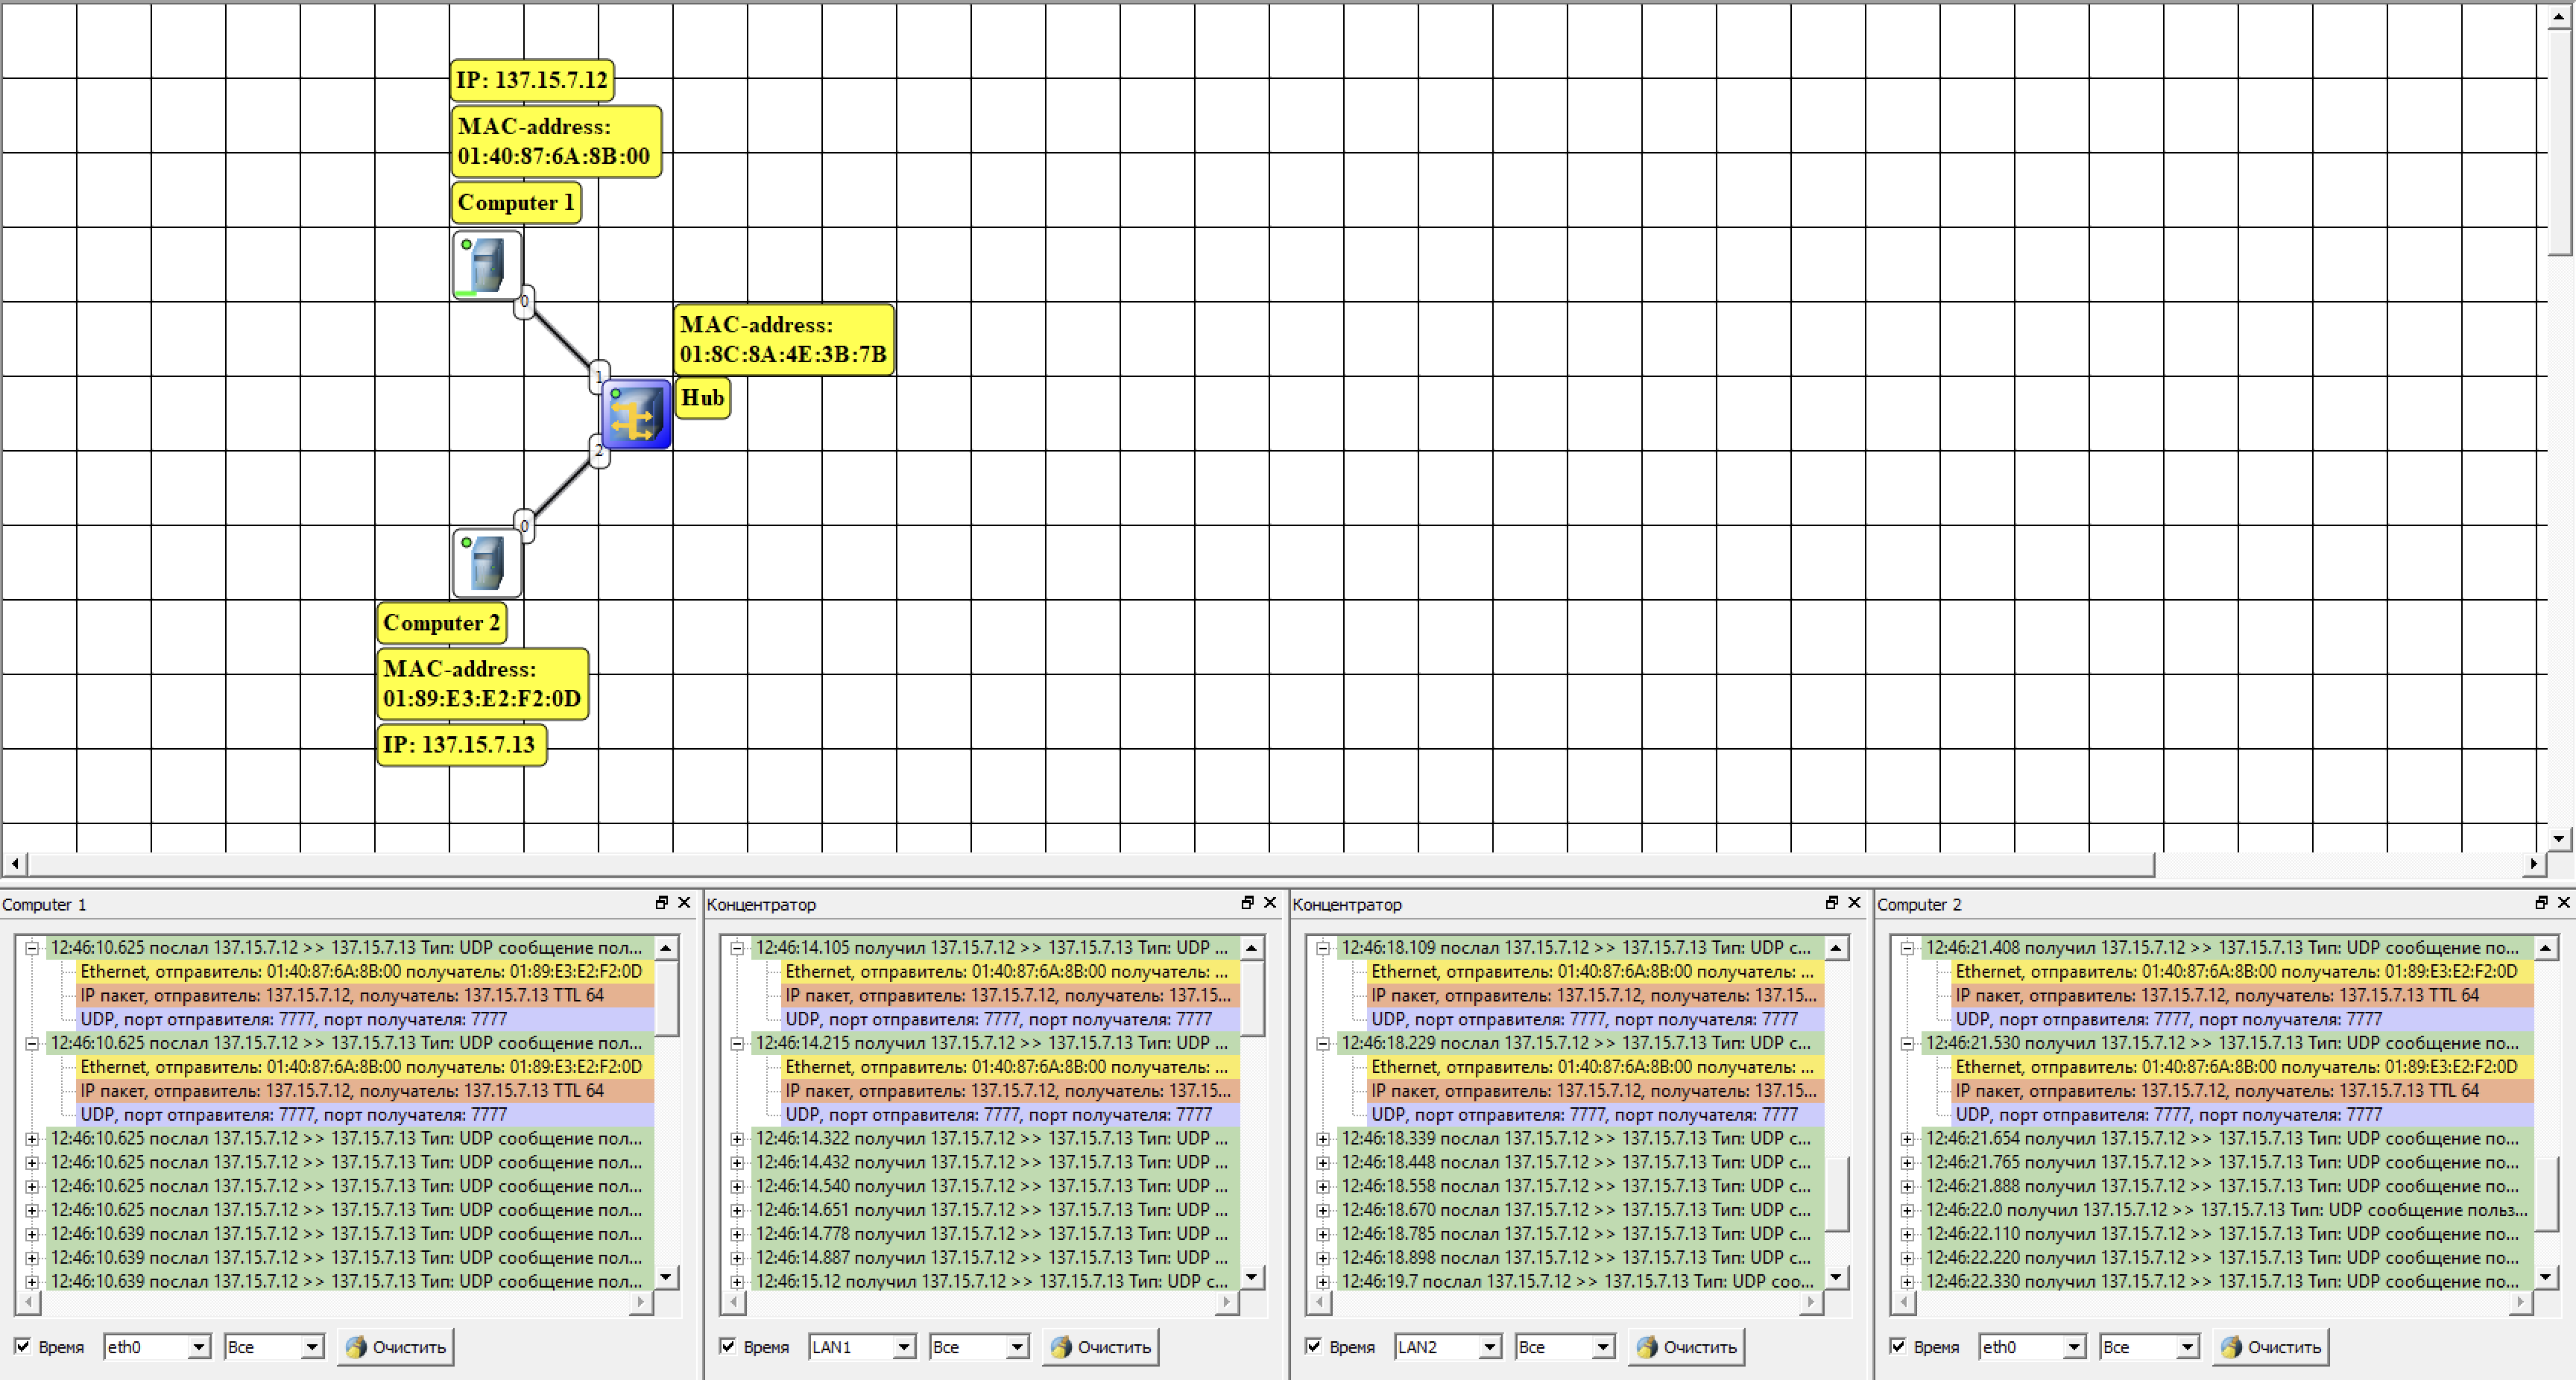
\includegraphics[width=\textwidth]{image/part1/udp-1.png}
  \caption{Отправка UDP-пакета с компьютера 1 на компьютер 2}
\end{figure}
По сети передается UPD датаграмма. UPD не требуется установки
соединения. Последовательность пакетов и кадров (сверху-вниз оборачивание):
Ethernet кадр с МАС адресами отправителя и получателя, IP пакет с IP адресами
отправителя и получателя и флагами (TTL - максимальное количество
«прыжков», что пакет должен существовать внутри сети, прежде чем он будет
отброшен маршрутизатором), UDP датаграмма с портами отправителя и
получателя.

Благодаря записям в ARP-таблицах заполнено поле Ethernet с MAC-адресами отправителя и получателя.

Последовательность отправки датаграмм в UDP не гарантируется.

Если бы у нас было бы больше двух компьютеров, то мы бы заметили, что датаграммы дошли до всех компьютеров кроме отправителя. Это происходит потому, что концентратор широковещательно отправляет все пакеты на все порты, кроме того, на котором он получил пакет.
Предполагается, что остальные компьютеры должны отбросить пакет, так как MAC-адрес получателя не совпадает с их собственным MAC-адресом.

\subsubsection{TCP}
\begin{figure}[H]
  \centering
  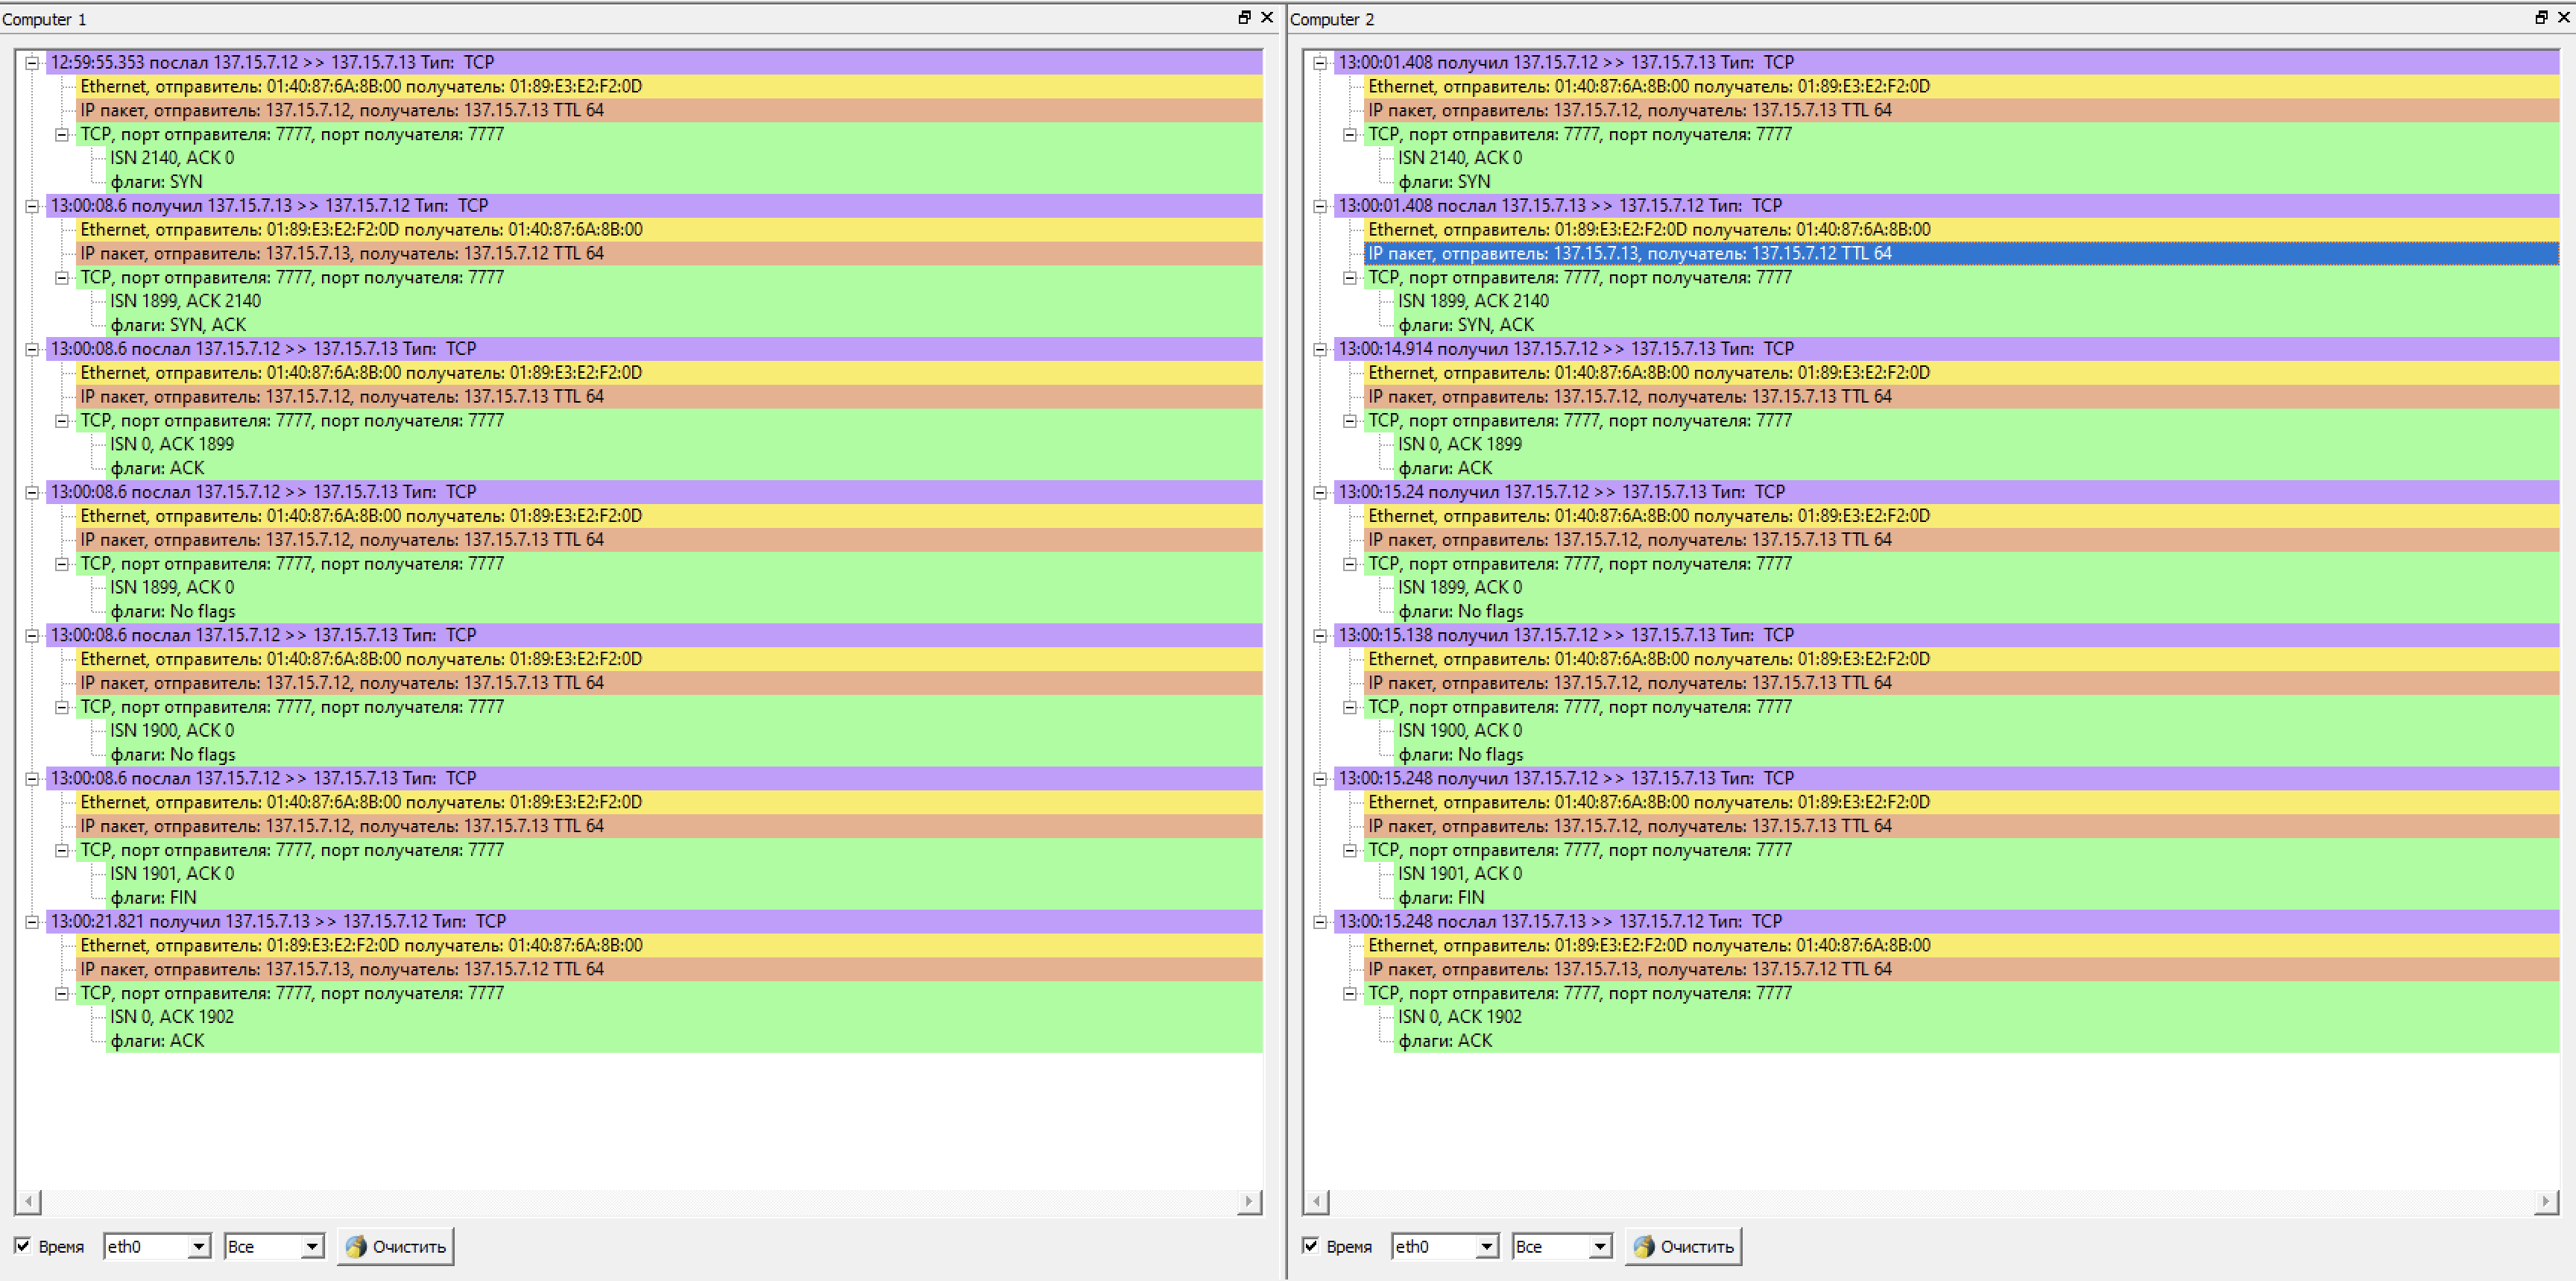
\includegraphics[width=\textwidth]{image/part1/tcp.png}
  \caption{Отправка TCP-пакета с компьютера 1 на компьютер 2}
\end{figure}

При отправке по TCP, сначала устанавливается соединение между отправителем и получателем. После этого отправляются данные. После передачи данных соединение закрывается.

Сначала происходит установка соединения: Компьютер 1 отправляет пакет с флагом SYN (синхронизация) на Компьютер 2, при этом сегменту присваивается порядковый номер ISN 2140. Относительно порядкового номера будет вестись отчет сегментов. Компьютер 2 отвечает пакетом с флагами SYN и ACK (подтверждение), а также установливает свой порядковый номер ISN 1899 и ACK (Acknowledgment - порядковый номер, который источник ожидает получить от получателя в следующий раз). Компьютер 1 отправляет пакет с флагом ACK. Теперь соединение установлено.

Далее Компьютер 1 отправляет Компьютеру 2 3Кбайта данных, после чего следует сегмент с флагом FIN (разрыв соединения). Компьютер 2 отвечает пакетом с флагом ACK (подтверждение приема). Теперь соединение закрыто.

Пакет содержит: Ethernet кадр с МАС-адресами
отправителя и получателя, IP пакет с IP адресами отправителя и получателя,
TCP пакет с портами отправителя и получателя, флагами, переменными (АСК,
ISN) и т.д.
\subsubsection{Вывод}

Основное различие между TCP и UDP заключается в том, что TCP устанавливает соединение и гарантирует доставку и порядок пакетов с помощью метаданных в заголовке TCP-пакета, а UDP - нет. Это означает, что UDP работает быстрее, потому что у него меньше метаданных и он не требует подтверждений, а также несет меньше накладных расходов в виде флагов и переменных.

\section{Локальная сеть с коммутатором (Сеть 2)}
\subsection{Построение локальной сети с коммутатором.}
Построил сеть из трех компьютеров и коммутатора.
\begin{figure}[H]
  \centering
  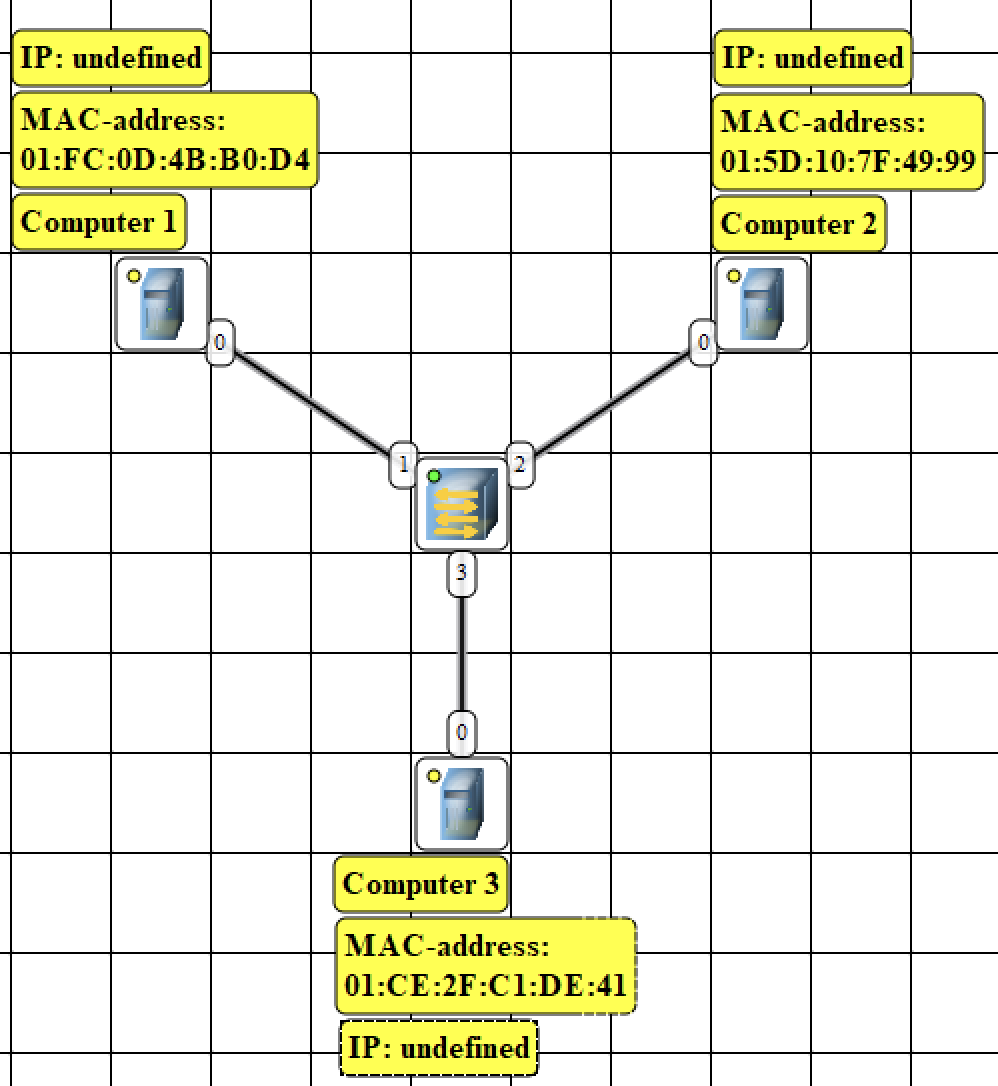
\includegraphics[width=\textwidth]{image/part2/topology.png}
  \caption{Схема сети из трех компьютеров и коммутатора}
\end{figure}

Изначально таблица коммутации пустая.
\begin{figure}[H]
  \centering
  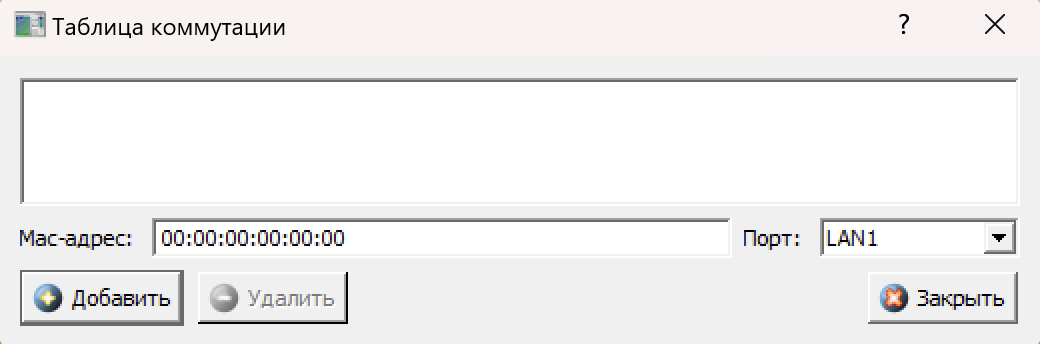
\includegraphics[width=\textwidth]{image/part2/switching-table.png}
  \caption{Таблица коммутации}
\end{figure}

Назначим IP-адреса компьютерам.
\begin{figure}[H]
  \centering
  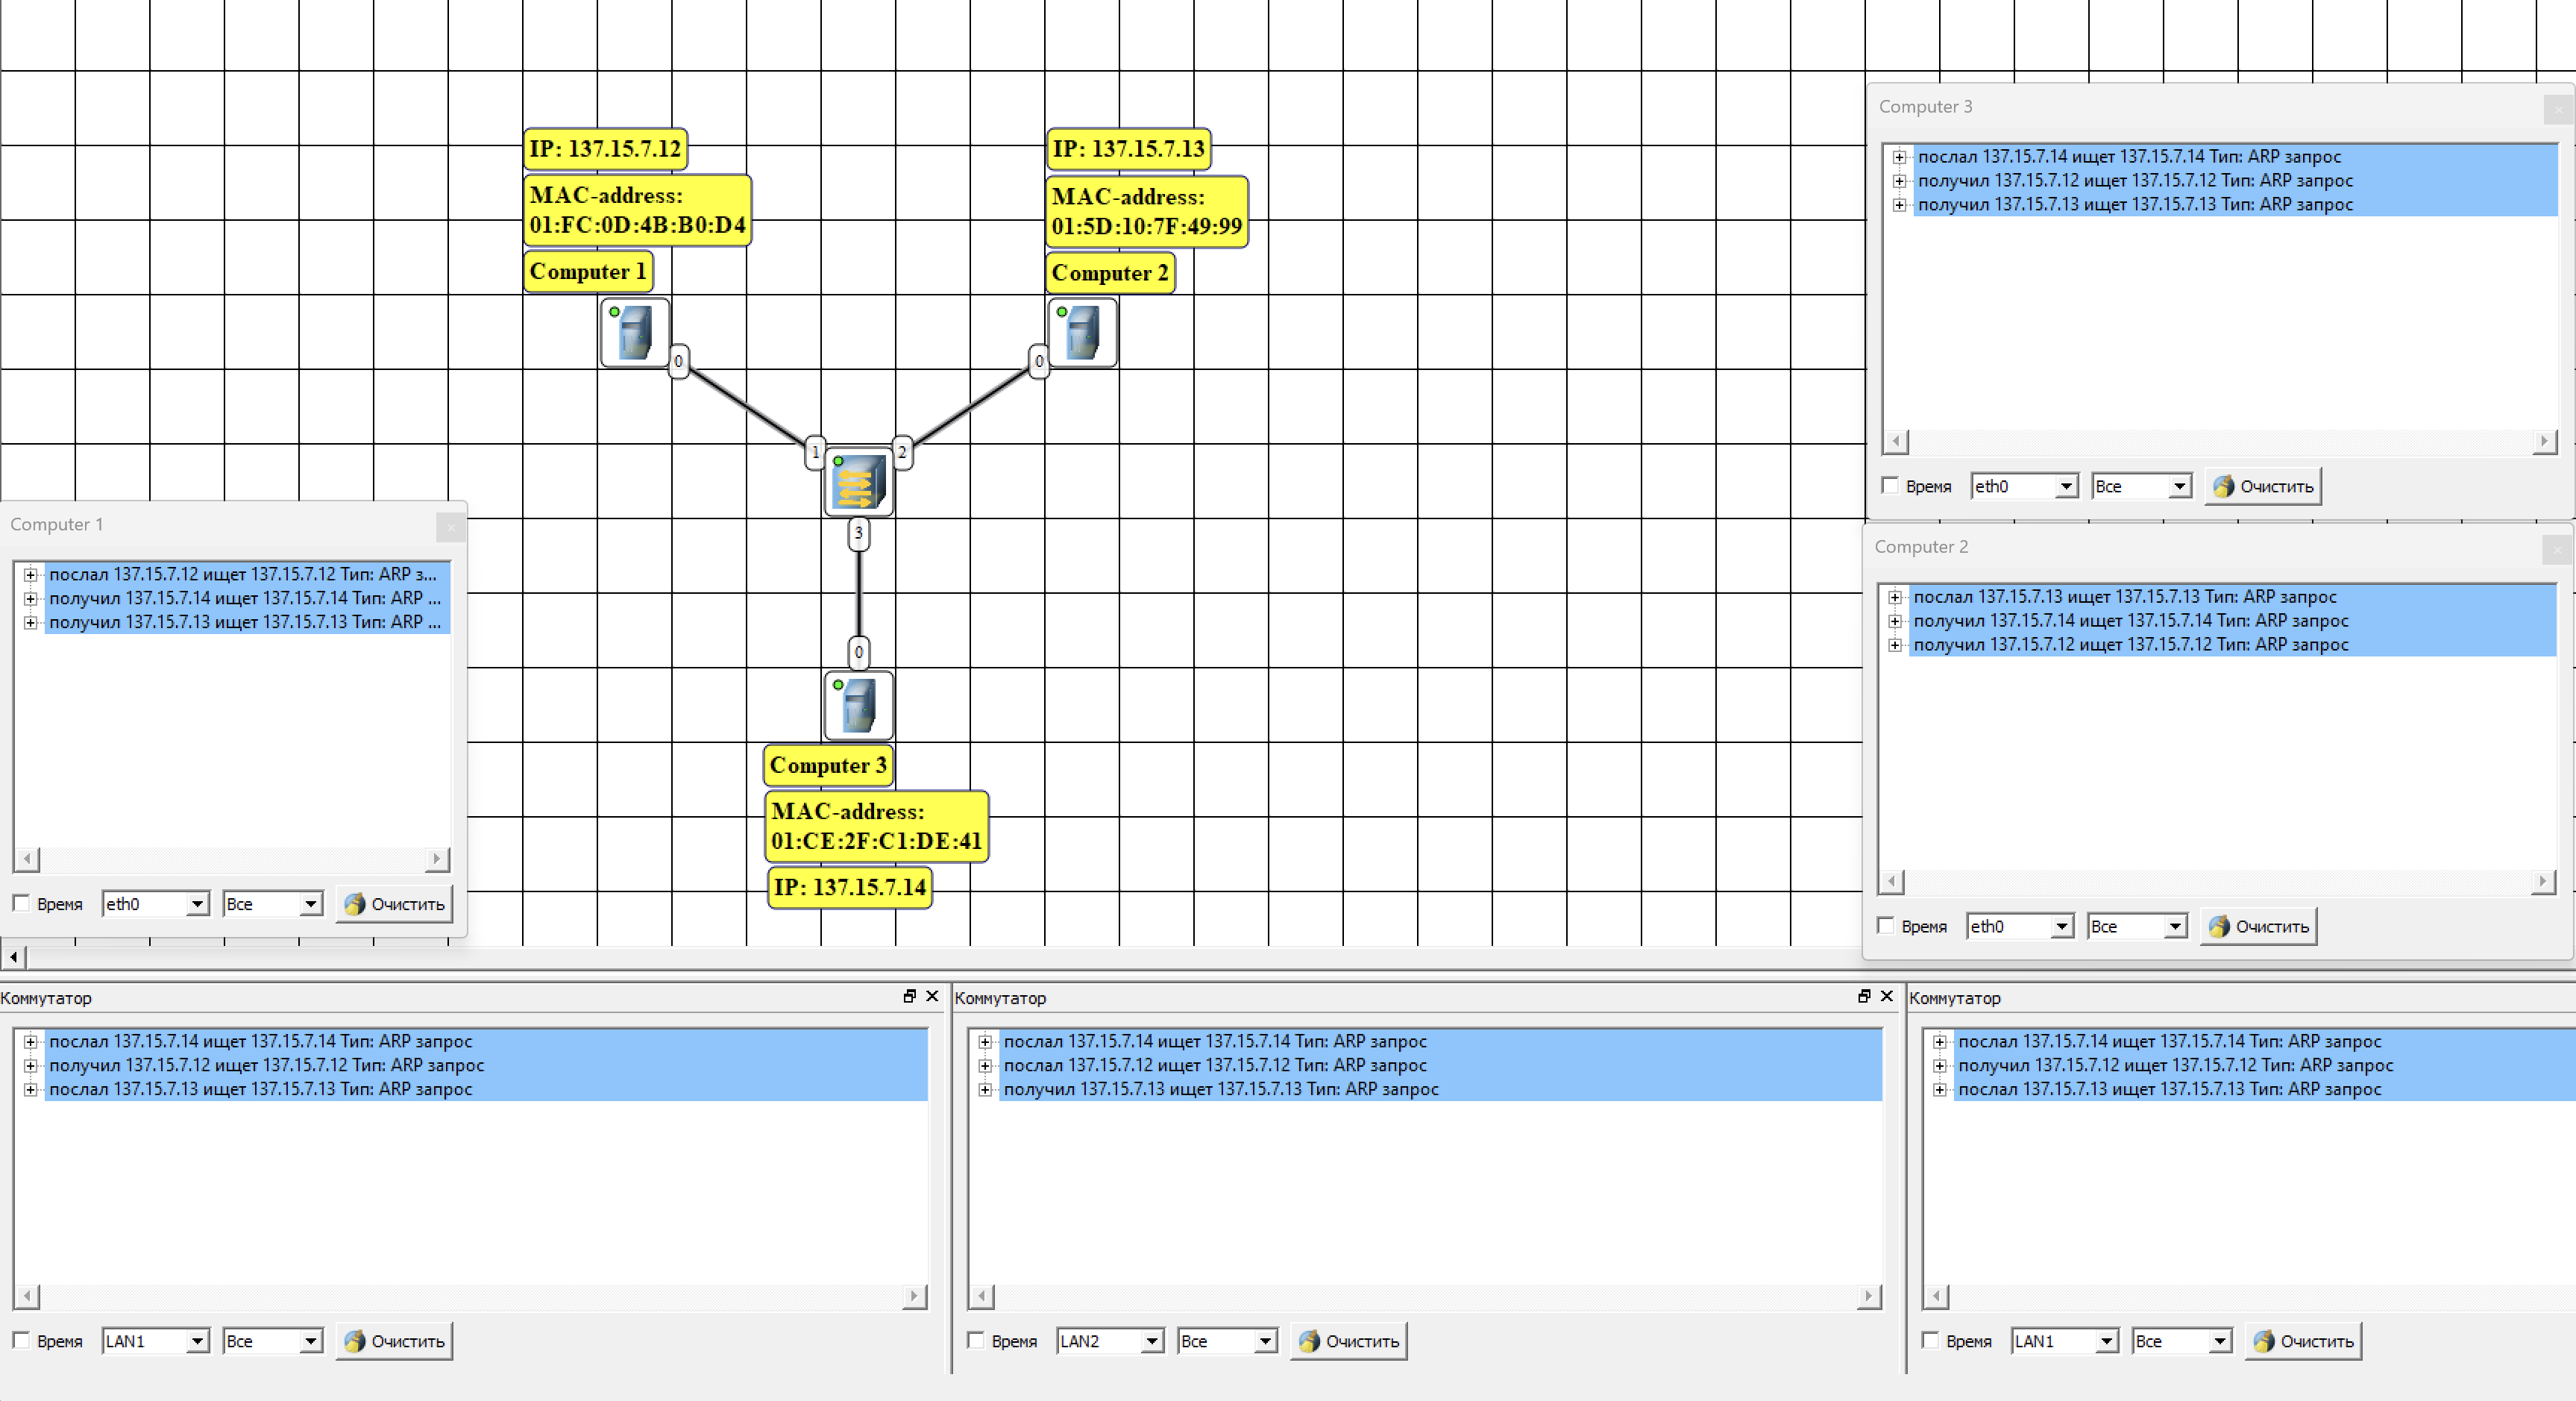
\includegraphics[width=\textwidth]{image/part2/topology-ip.png}
  \caption{Присвоение IP-адресов}
\end{figure}
Таблица коммутации будет заполнена благодаря отправляемым ARP-запросам:

\begin{figure}[H]
  \centering
  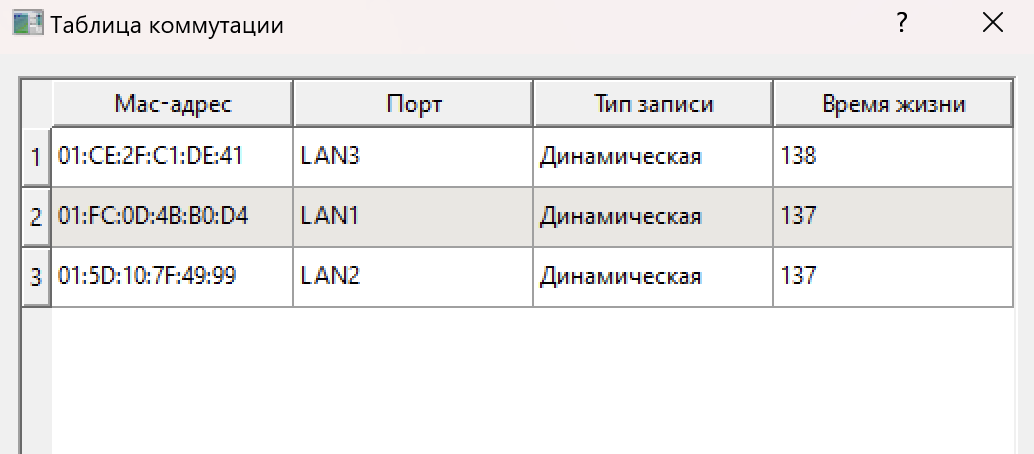
\includegraphics[width=\textwidth]{image/part2/switch-table.png}
  \caption{Таблица коммутации}
\end{figure}

Таблица коммутации состоит из следующих полей:
\begin{itemize}
  \item MAC-адрес подключенного устройства
  \item Порт коммутатора, в который подключено данное устройство
  \item Тип записи: динамическая или статическая
  \item Время жизни записи. Запись удаляется, если устройство не отправляло пакеты в течение определенного лимита. Измеряется в секундах. (По умолчанию TTL = 300 секунд)
\end{itemize}

\begin{itemize}
  \item {
    \textbf{Как происходит заполнение таблицы коммутации;}

    Когда компьютер отправляет пакет, коммутатор получает его и смотрит на MAC-адрес отправителя. Если запись с таким MAC-адресом уже есть в таблице, то коммутатор обновляет время жизни записи. Если записи нет, то коммутатор добавляет новую запись в таблицу.
  }
  \item {
    \textbf{На основе анализа какой информации заполняется таблица коммутации;}

    Из Ethernet-кадра запроса коммутатор извлечет
    MAC-адрес компьютера-отправителя.
  }
  \item {
    \textbf{В чем основные отличия передачи сообщений в сети с коммутатором от сети с концентратором;}

    Коммутатор пересылает пакеты только на те порты, на которых находится получатель, в то время как концентратор широковещательно отправляет пакеты на все порты, кроме того, на котором он получил пакет.

    Коммутаторы работают на канальном уровне модели OSI, а концентраторы - на физическом.

    Когда коммутатор включается, он начинает работу в режиме обучения с пустой таблицей. В этом режиме входящие данные на любой порт передаются на все остальные порты (как концентратор). Коммутатор анализирует кадры и записывает MAC-адрес отправителя в таблицу. Если на порт приходит кадр, предназначенный для хоста с известным МАС-адресом, то он будет передан только через указанный порт. Если MAC-адрес хоста-получателя неизвестен, кадр будет продублирован на всех интерфейсах.

  }
  \item {
    \textbf{Когда (при каком условии) таблица коммутации будет построена полностью;}

    Таблица коммутации будет полностью построена, когда все компьютеры отправят запросы и эти запросы попадут в таблицу коммутации, и не пройдет для какого-либо из них максимальное время жизни. 
  }

  \item {
    \textbf{Чему равно максимальное количество записей (строк) в таблице коммутации.}

    К одному порту может быть привязано несколько
    различных МАС адресов. 
    Максимальное количество строк в таблице зависит от модели коммутатора и, возможно,
прошивки.
  }
\end{itemize}

\subsection{Анализ таблиц.}
\begin{figure}[H]
  \centering
  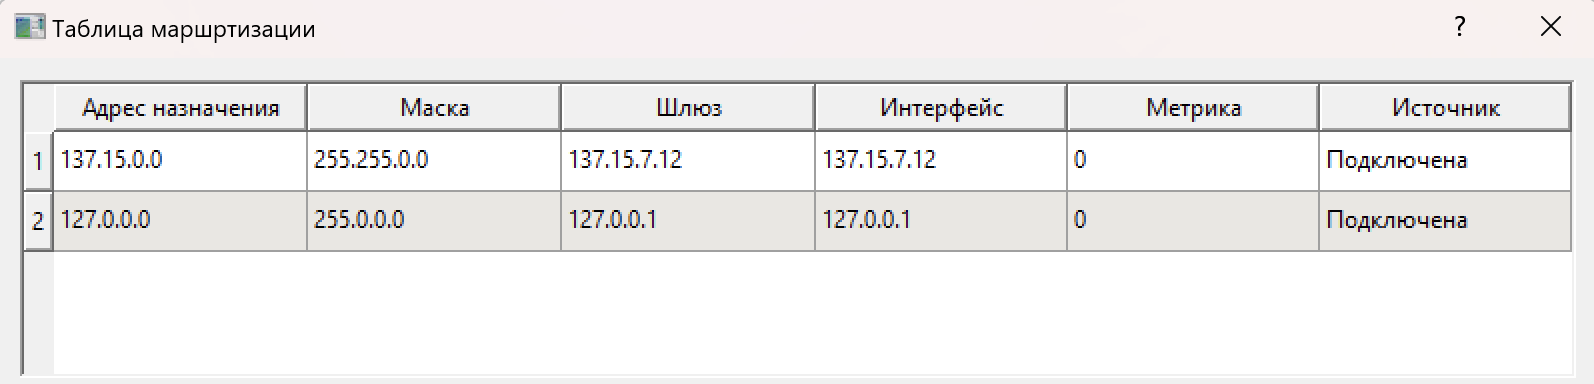
\includegraphics[width=\textwidth]{image/part2/routing-table.png}
  \caption{Таблица маршрутизации компьютера 1}
\end{figure}
\begin{figure}[H]
  \centering
  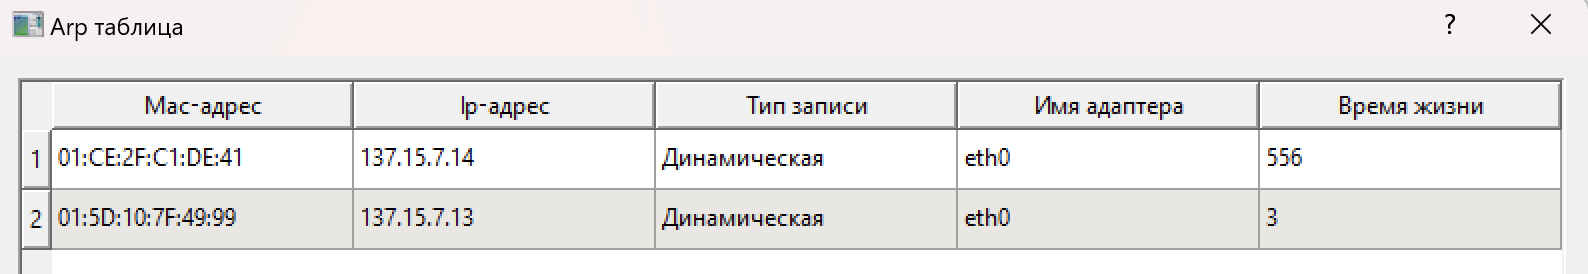
\includegraphics[width=\textwidth]{image/part2/arp-table.png}
  \caption{Таблица ARP компьютера 1}
\end{figure}

Таблицы маршрутизации изменились аналогичным образом, как и при передаче через концентратор.

Появились новые записи в Агр-таблице после отправки Агр-запросов.

\subsection{Тестирование сети (отправка пакетов).}

\subsubsection{UDP}
\begin{figure}[H]
  \centering
  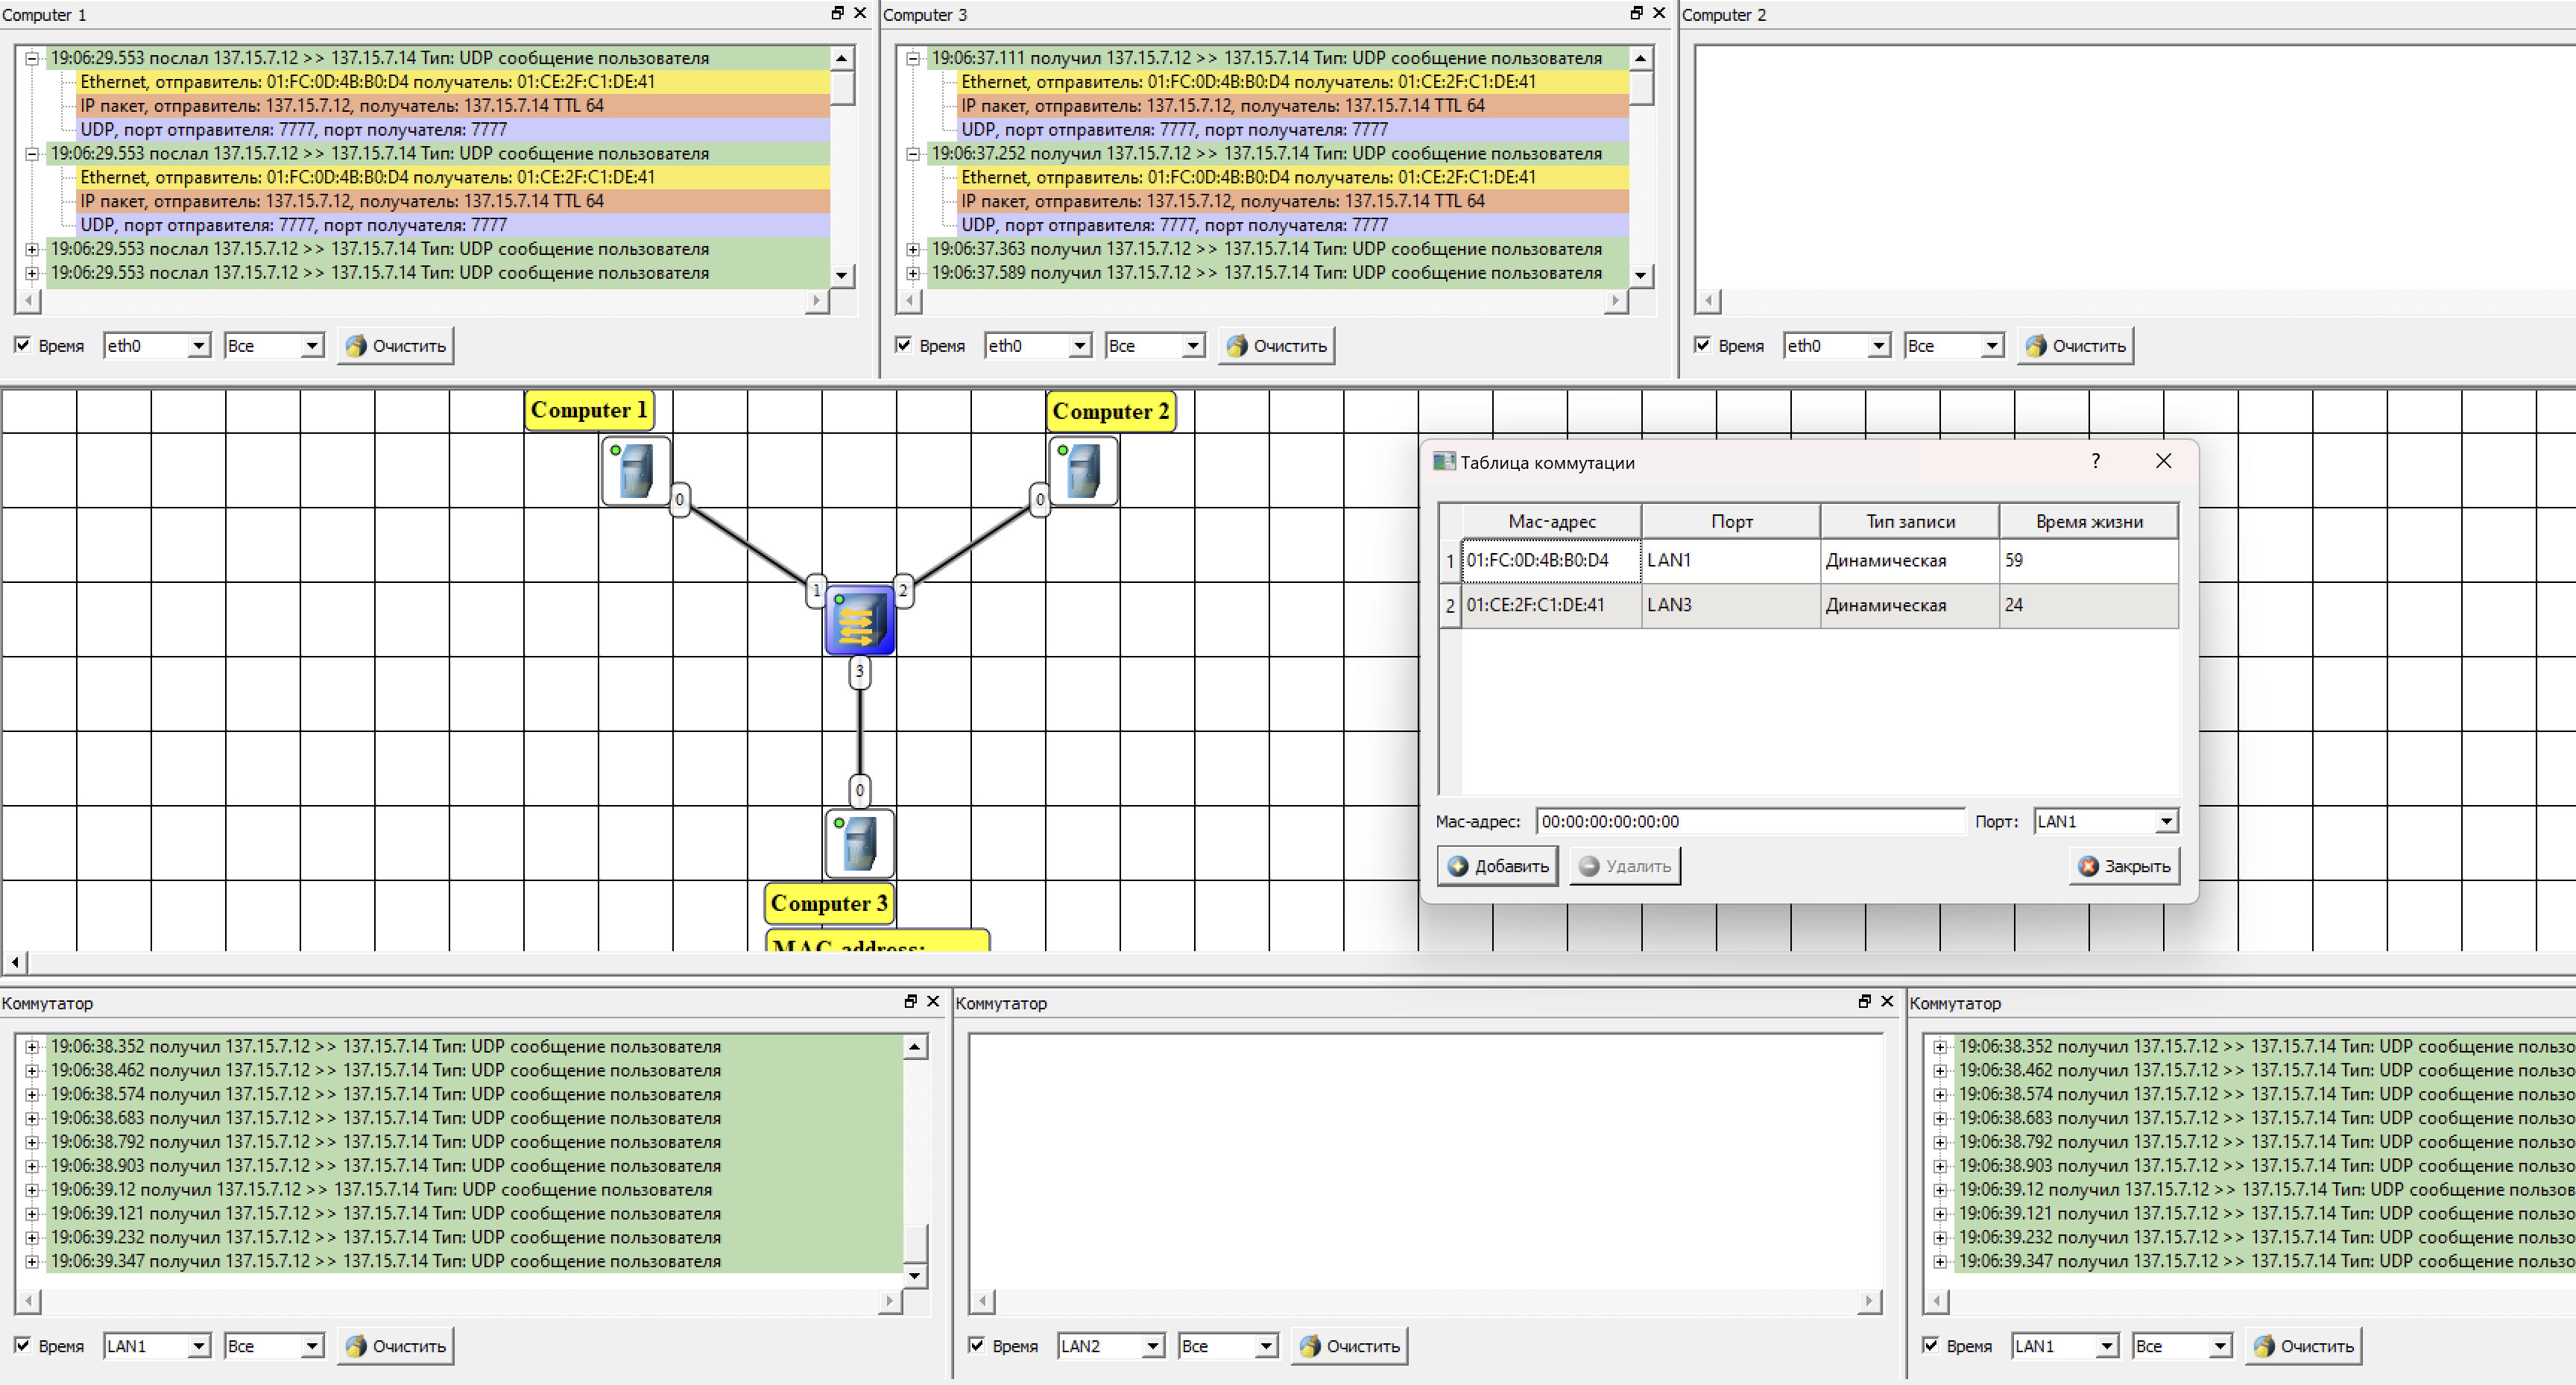
\includegraphics[width=\textwidth]{image/part2/udp.png}
  \caption{Отправка UDP-пакета с компьютера 1 на компьютер 3}
\end{figure}

Последовательность пакетов их содержание аналогичны отправке через концентратор.

Таблицы маршрутизации не изменились.

В ARP-таблицах появились записи об отправителе на получателе (и наоборот).

Главное отличие с концентратором заключается в том, что так как таблица коммутации на коммутаторе заполнена, то пакеты не были отправлены на все порты, а только на тот, на котором находится получатель.

\subsubsection{TCP}
\begin{figure}[H]
  \centering
  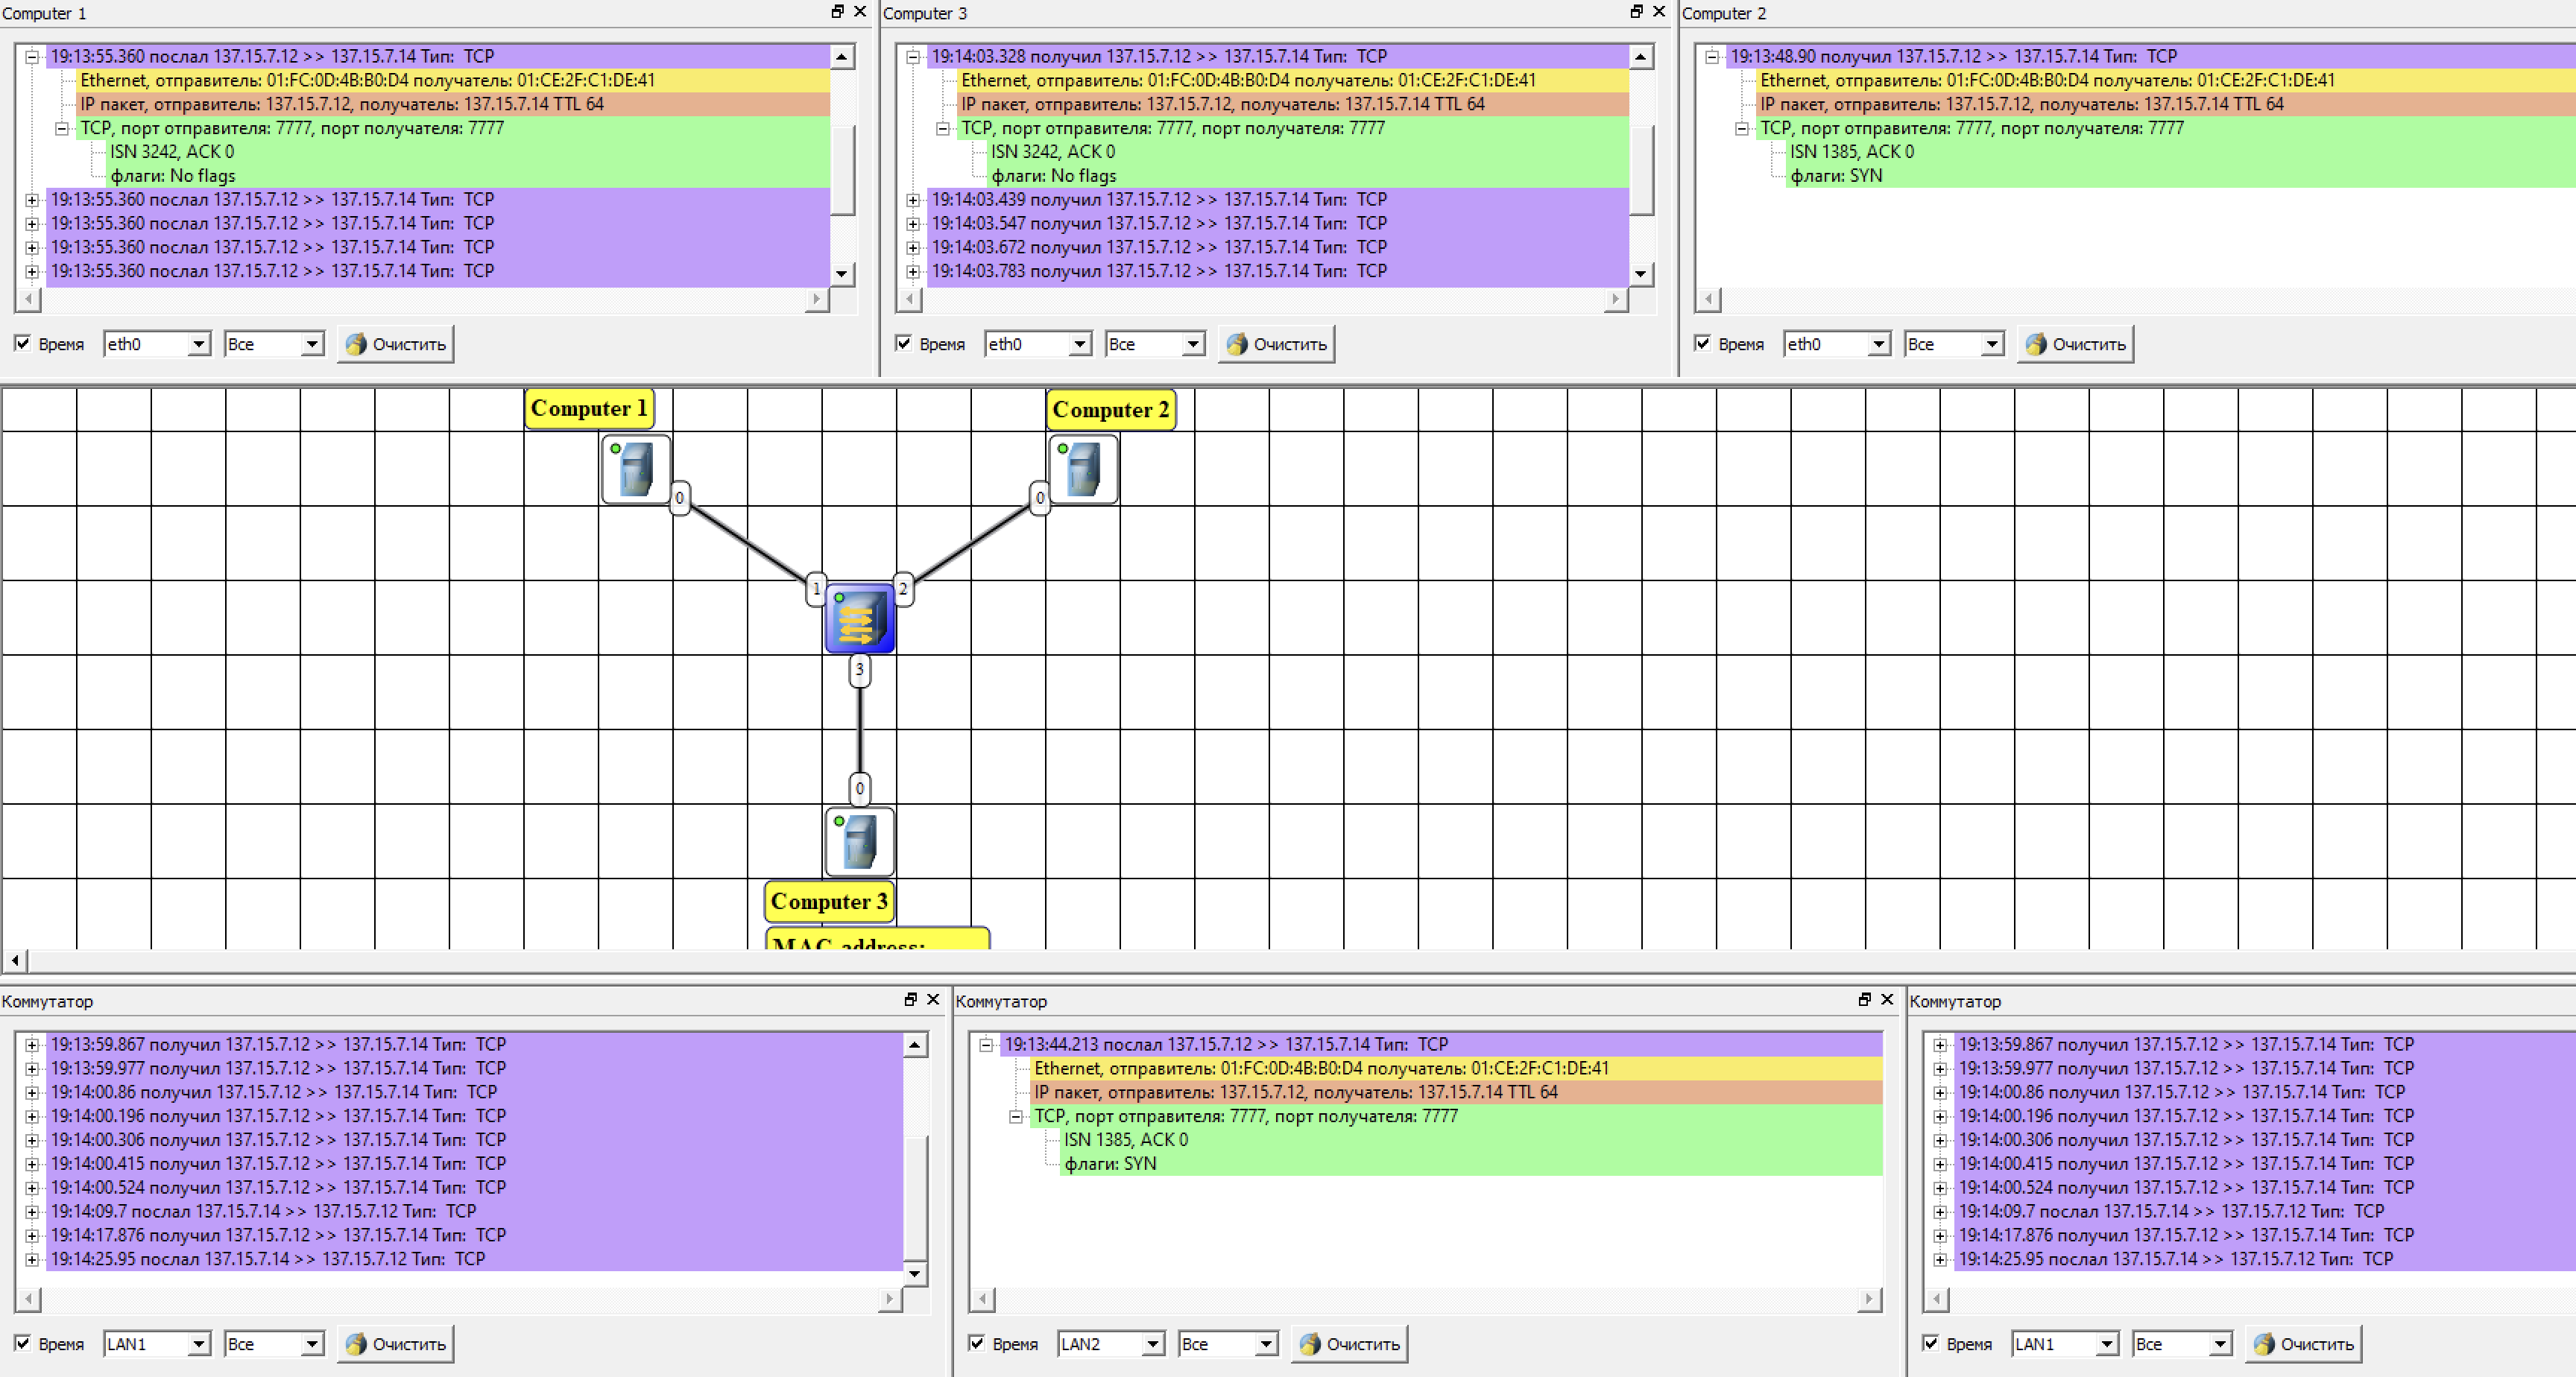
\includegraphics[width=\textwidth]{image/part2/tcp.png}
  \caption{Отправка TCP-пакета с компьютера 1 на компьютер 3}
\end{figure}

Последовательность пакетов и их содержание аналогичны отправке через концентратор.

Таблицы маршрутизации не изменились.

В ARP-таблицах появились записи об отправителе на получателе (и наоборот).

В отличие от концентратора, коммутатор при отсутствии записи о получателе отправит на все порты только первый SYN-запрос. Затем все последующие пакеты будут отправляться только на порт, где находится получатель, так как к тому времени запись о нем появится в таблице коммутации.

\section{Многосегментная локальная сеть (Сеть 3)}
\subsection{Формирование сети.}
Содержимое Агр-таблиц и таблицы маршрутизации почти не изменилось.

В таблице коммутации появилось больше записей, которые относятся к одному порту, но при этом с разными МАС-адресами. Такое происходит из-за того, что коммутаторы
объединены с другими коммутаторами или концентраторами, которые объединяют
несколько компьютеров.

\begin{figure}[H]
  \centering
  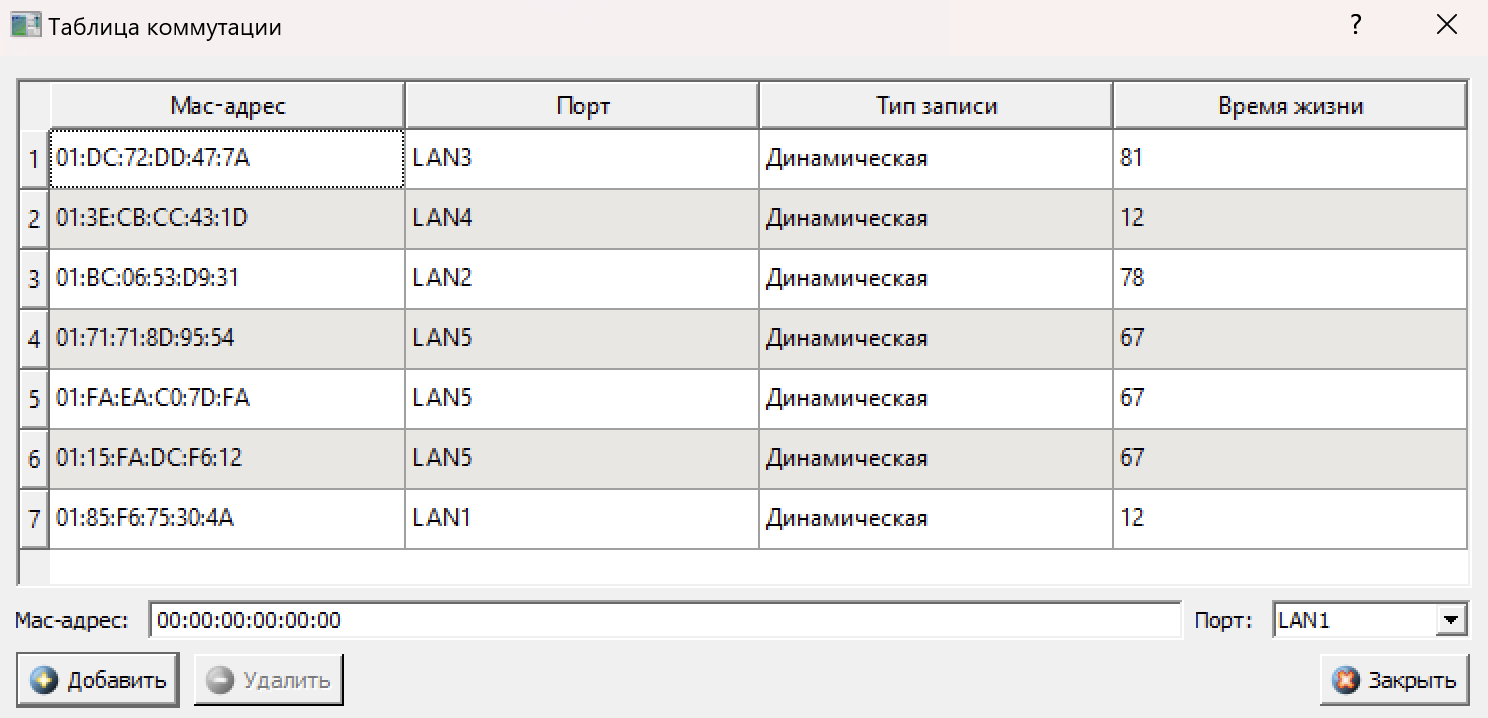
\includegraphics[width=\textwidth]{image/part3/switch-table-1.png}
  \caption{Таблица коммутации коммутатора 1}
\end{figure}
\begin{figure}[H]
  \centering
  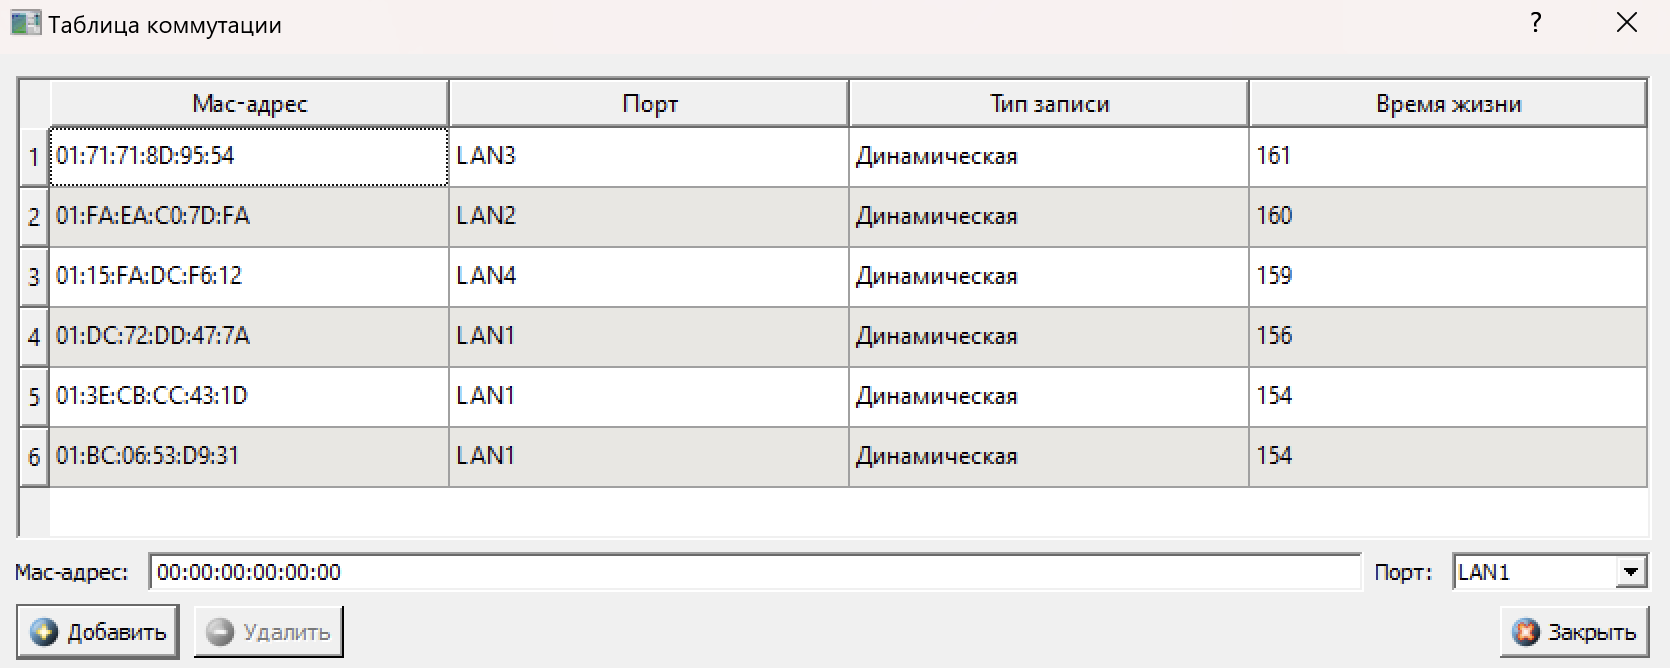
\includegraphics[width=\textwidth]{image/part3/switch-table-2.png}
  \caption{Таблица коммутации коммутатора 2}
\end{figure}
\subsection{Топология общая шина}
\begin{figure}[H]
  \centering
  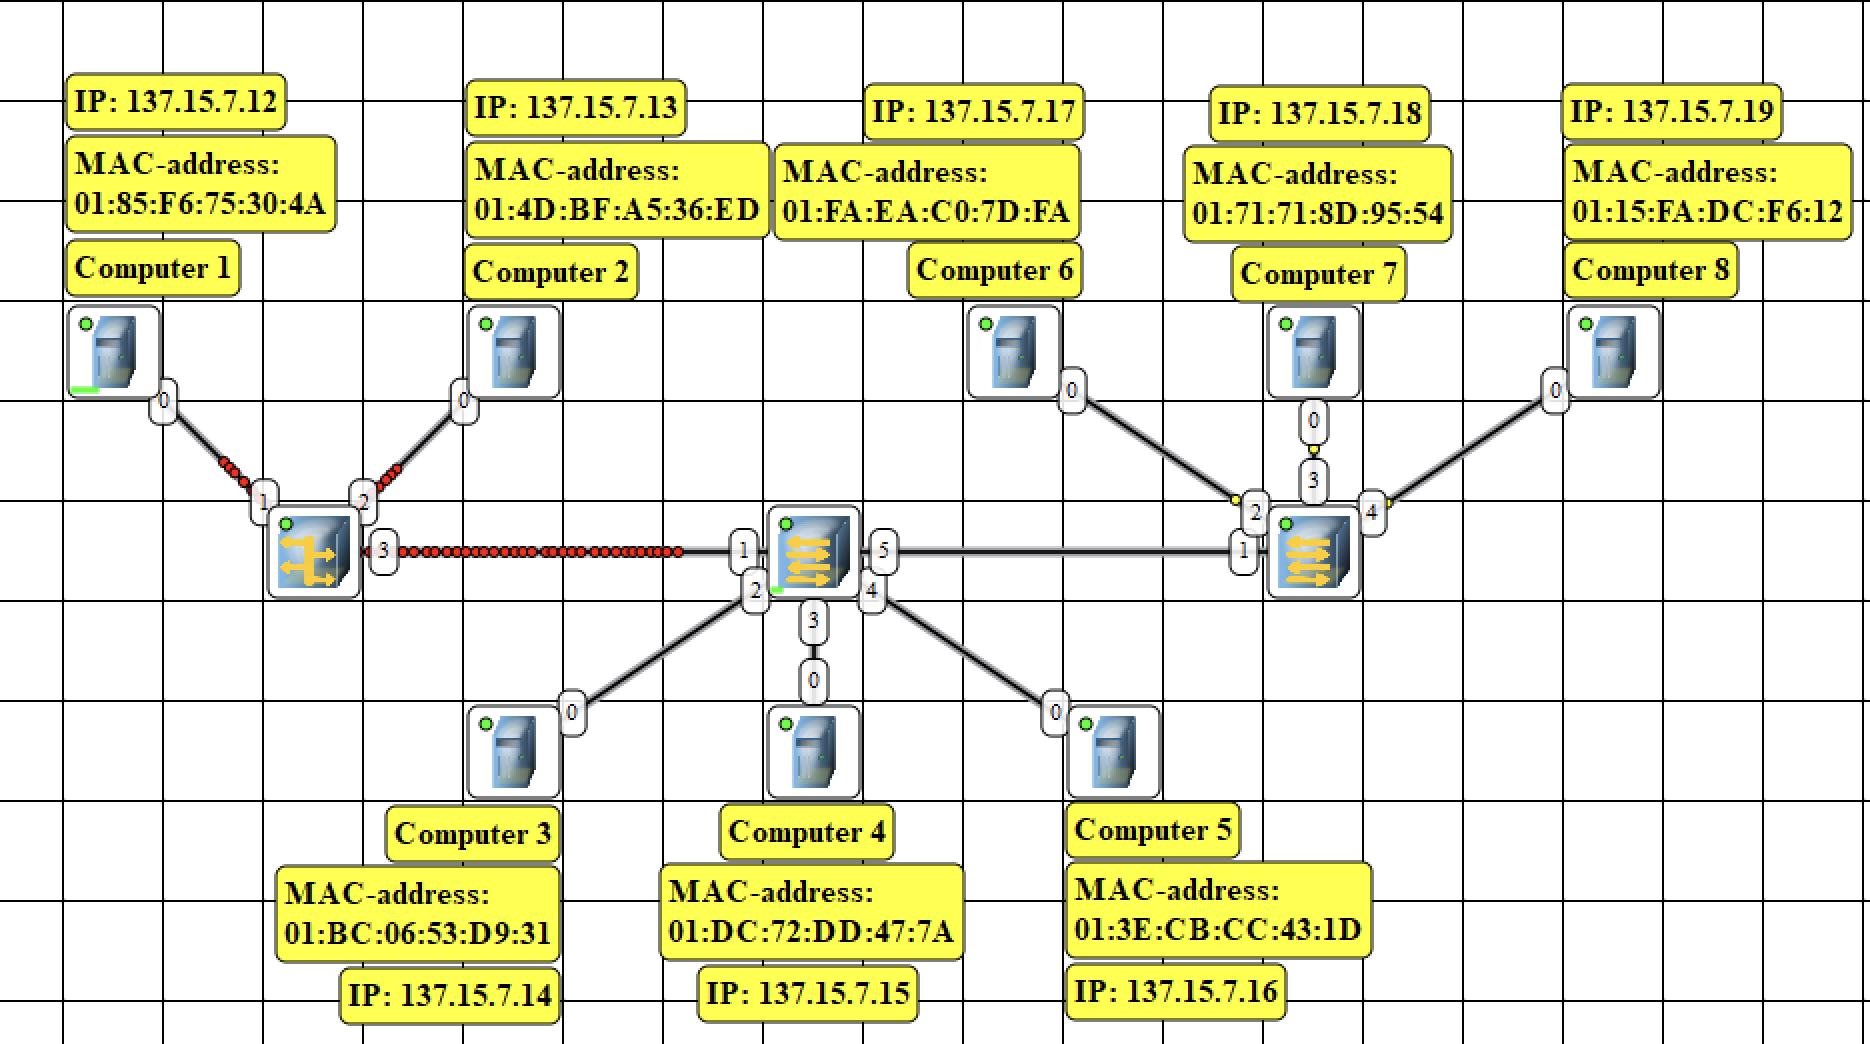
\includegraphics[width=\textwidth]{image/part3/shared-bus.png}
  \caption{Схема сети общая шина}
\end{figure}
Реализуема. Если таблицы маршрутизации внутри подсети с концентратором заполнены, отправка сообщений невозможна (UPD -- передает и сам себе тоже, TCP -- ломается при попытке установить соединение ). Если заменить концентратор на коммутатор, эта ошибка исчезнет. Также возможна реализация при использовании только концентраторов, но следует учитывать, что отправка одного сообщения может заполнить всю сеть, независимо от местонахождения его получателя.
\subsection{Топология кольцо}
\begin{figure}[H]
  \centering
  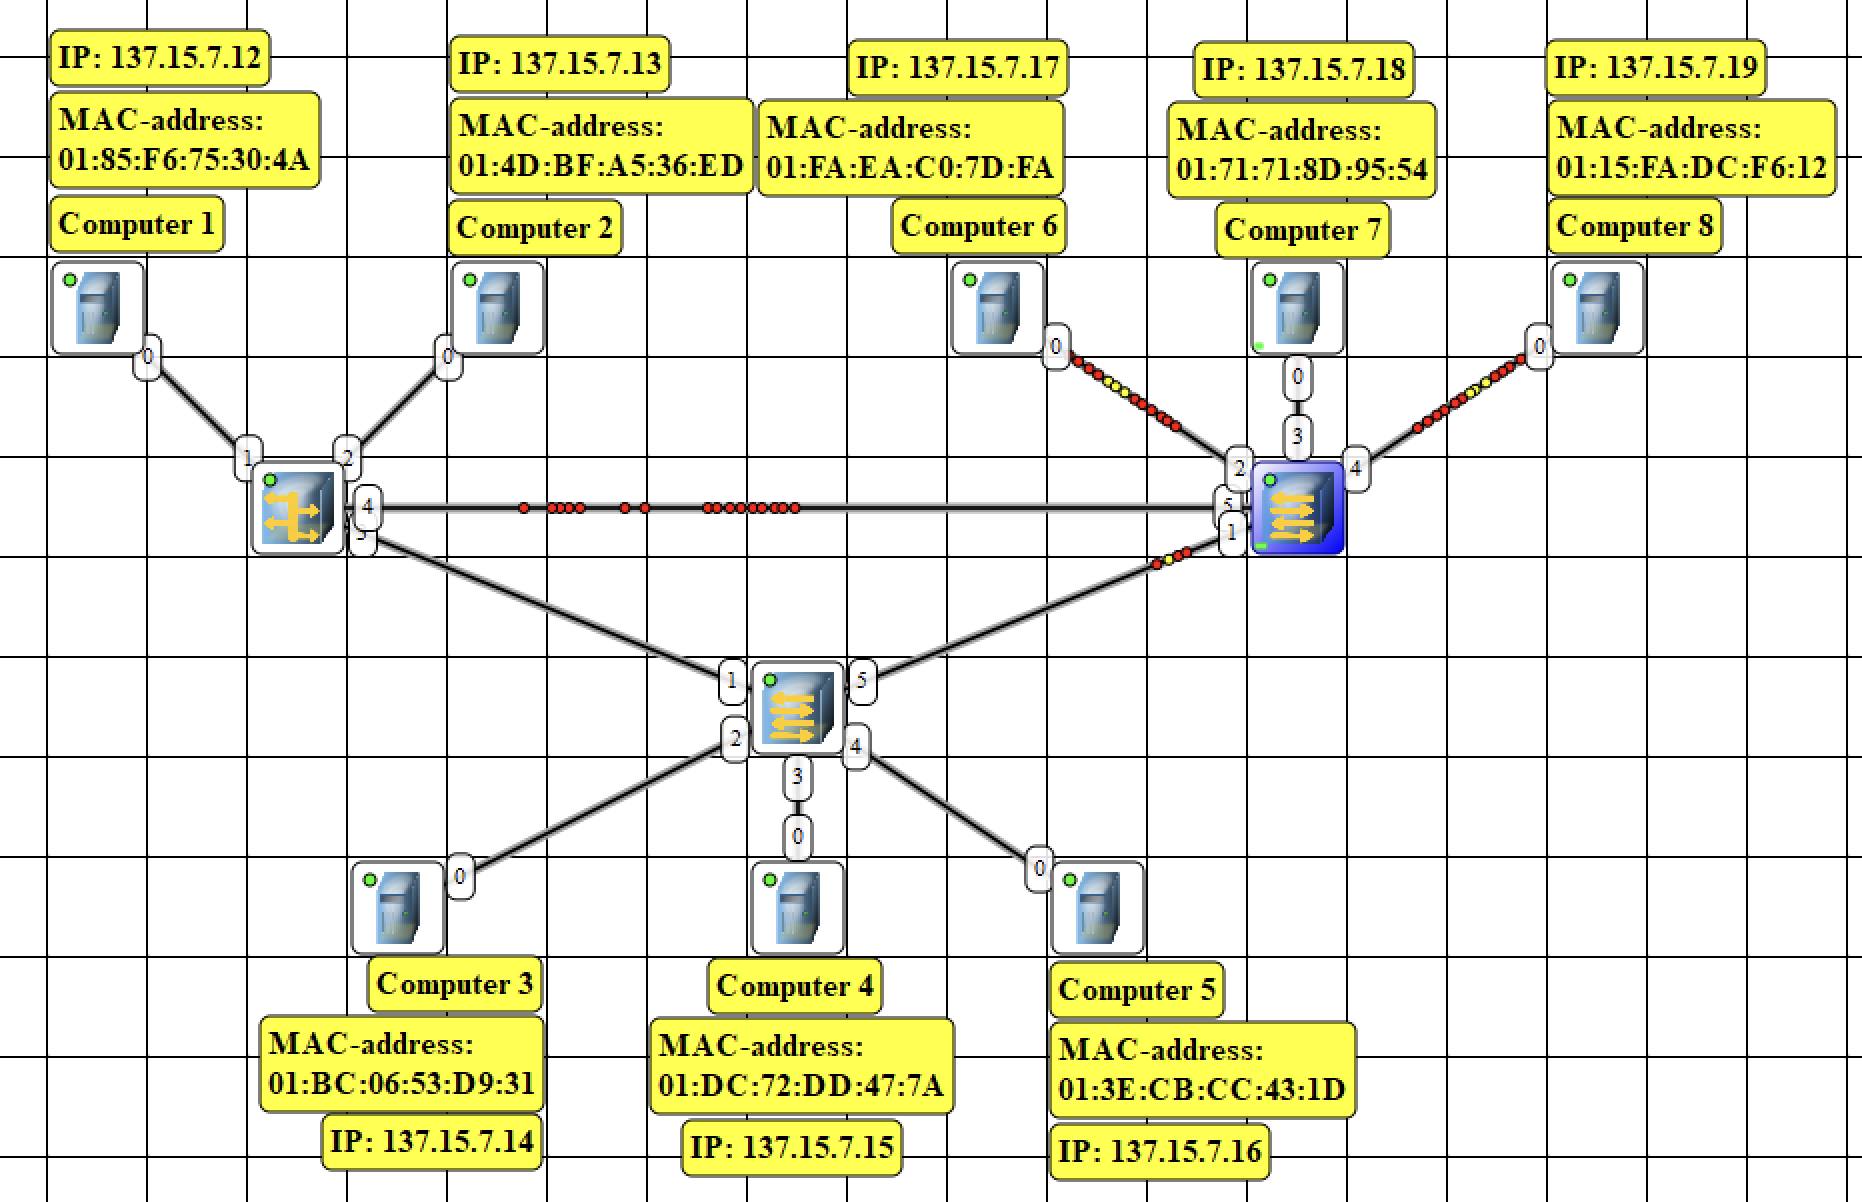
\includegraphics[width=\textwidth]{image/part3/ring.png}
  \caption{Схема сети кольцо}
\end{figure}
Нереализуема. Возникает циклическая перессылка пакетов внутри сети. Пакеты будут бесконечно передаваться между коммутаторами и концентратором, пока не истечет TTL. 

Даже если заменить концентратор на коммутатор, пакеты продолжат бесконечно передаваться по сети, так как до заполнения таблицы коммутации они будут отправляться аналогично тому, как это происходит в случае концентратора. 

\subsection{Топология звезда}
\begin{figure}[H]
  \centering
  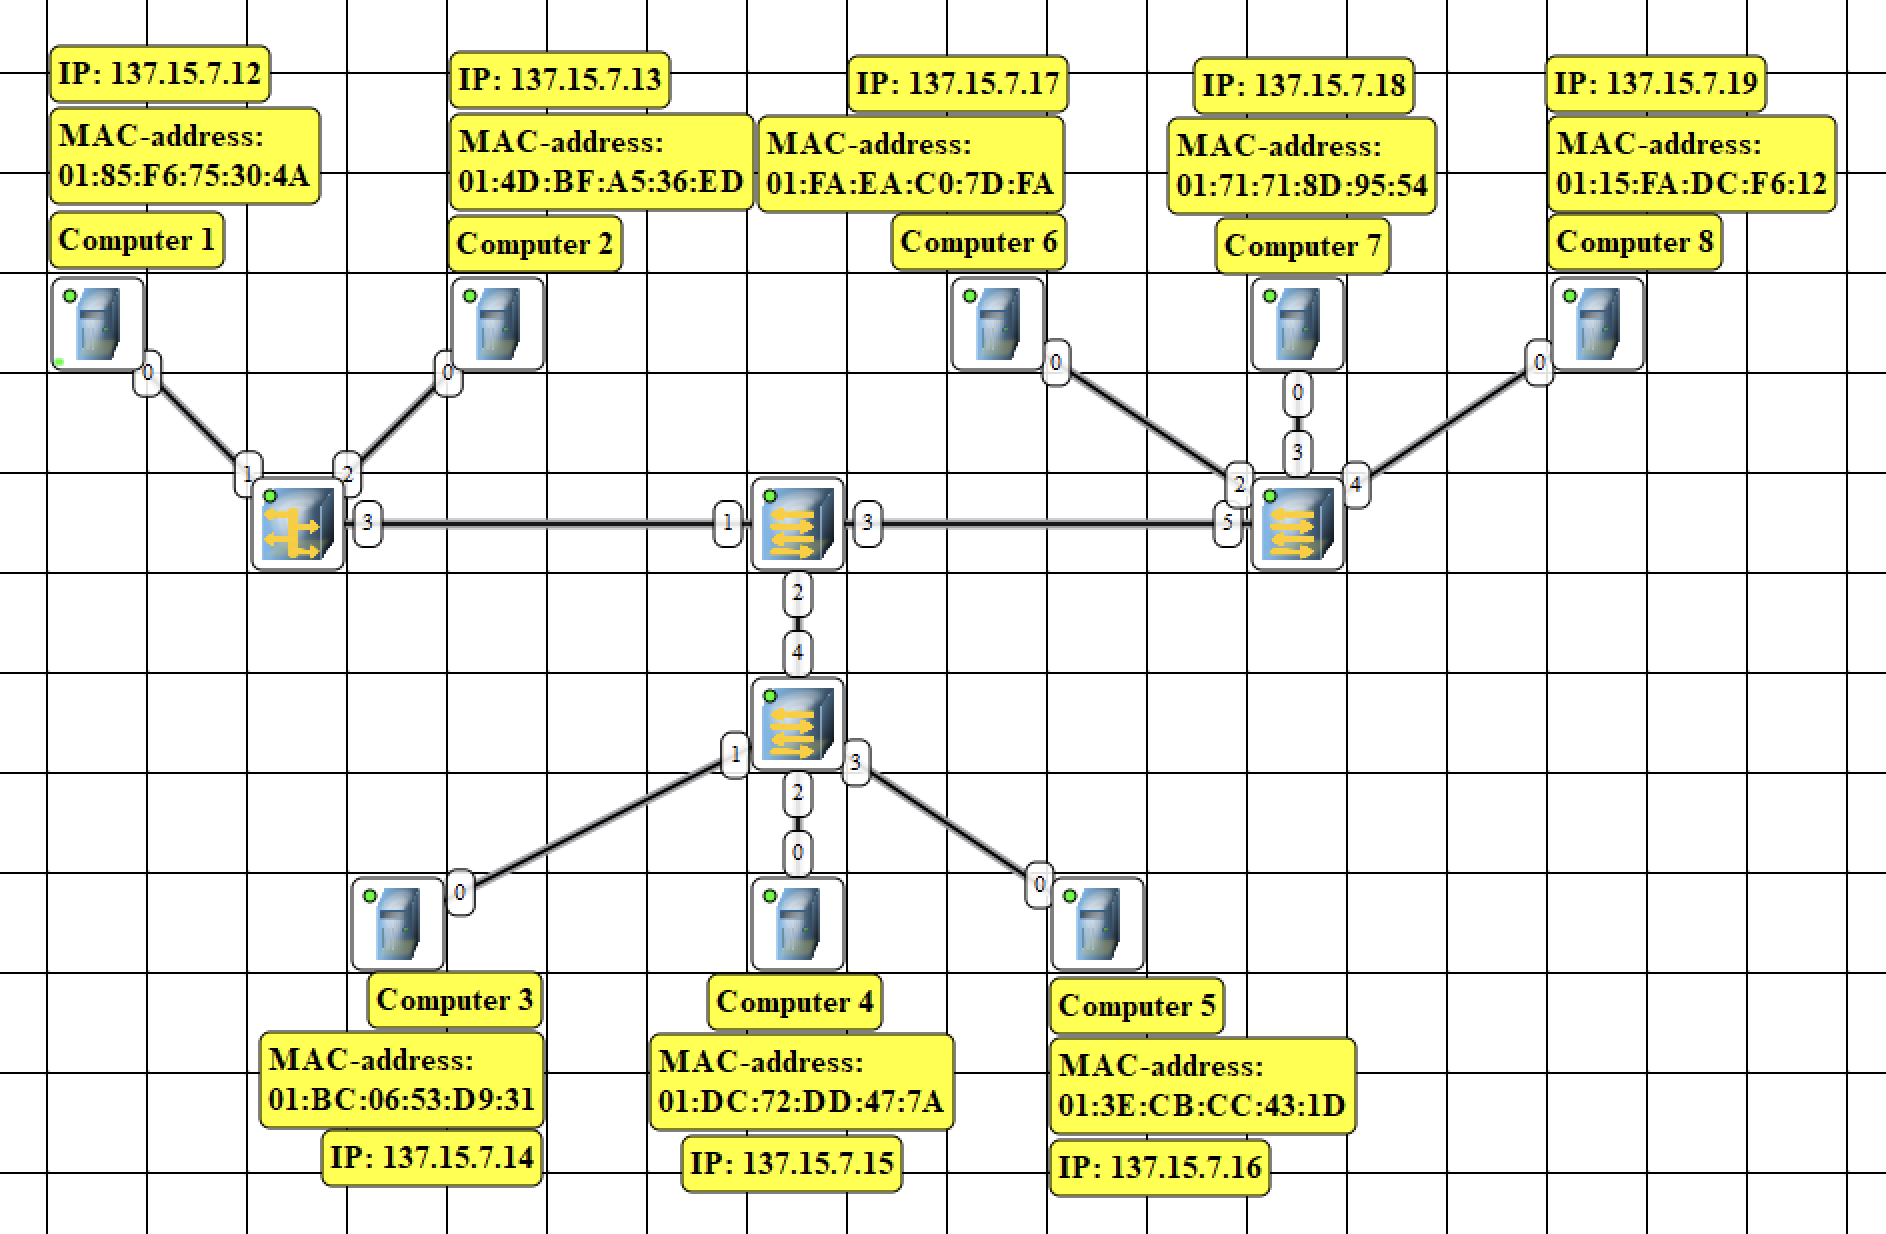
\includegraphics[width=\textwidth]{image/part3/star.png}
  \caption{Схема сети звезда}
\end{figure}

Реализуема. Также, как и в топологии общей шины, может дублировать сообщения при отправке внутри подсети с концентратором, но при замене его на коммутатор всё работает правильно. Также при замене коммутаторов на концентраторы всё работает корректно.

\subsubsection{Вывод}
Я думаю, что лучший вариант для такой конфигурации - топология "звезда" и общей шина. Если в сеть нужно будет добавить новые подсети, то топология "звезда" будет более удобной, потому что она уменьшает количество переходов сообщений между устройствами при подключении к общему маршрутизатору. Последующее тестирование будет проводиться для топологии "звезда"  с коммутаторами на всех сегментах и в точке соединения.

\subsection{Тестирование сети (отправка пакетов).}
\subsection{UDP}
\begin{figure}[H]
  \centering
  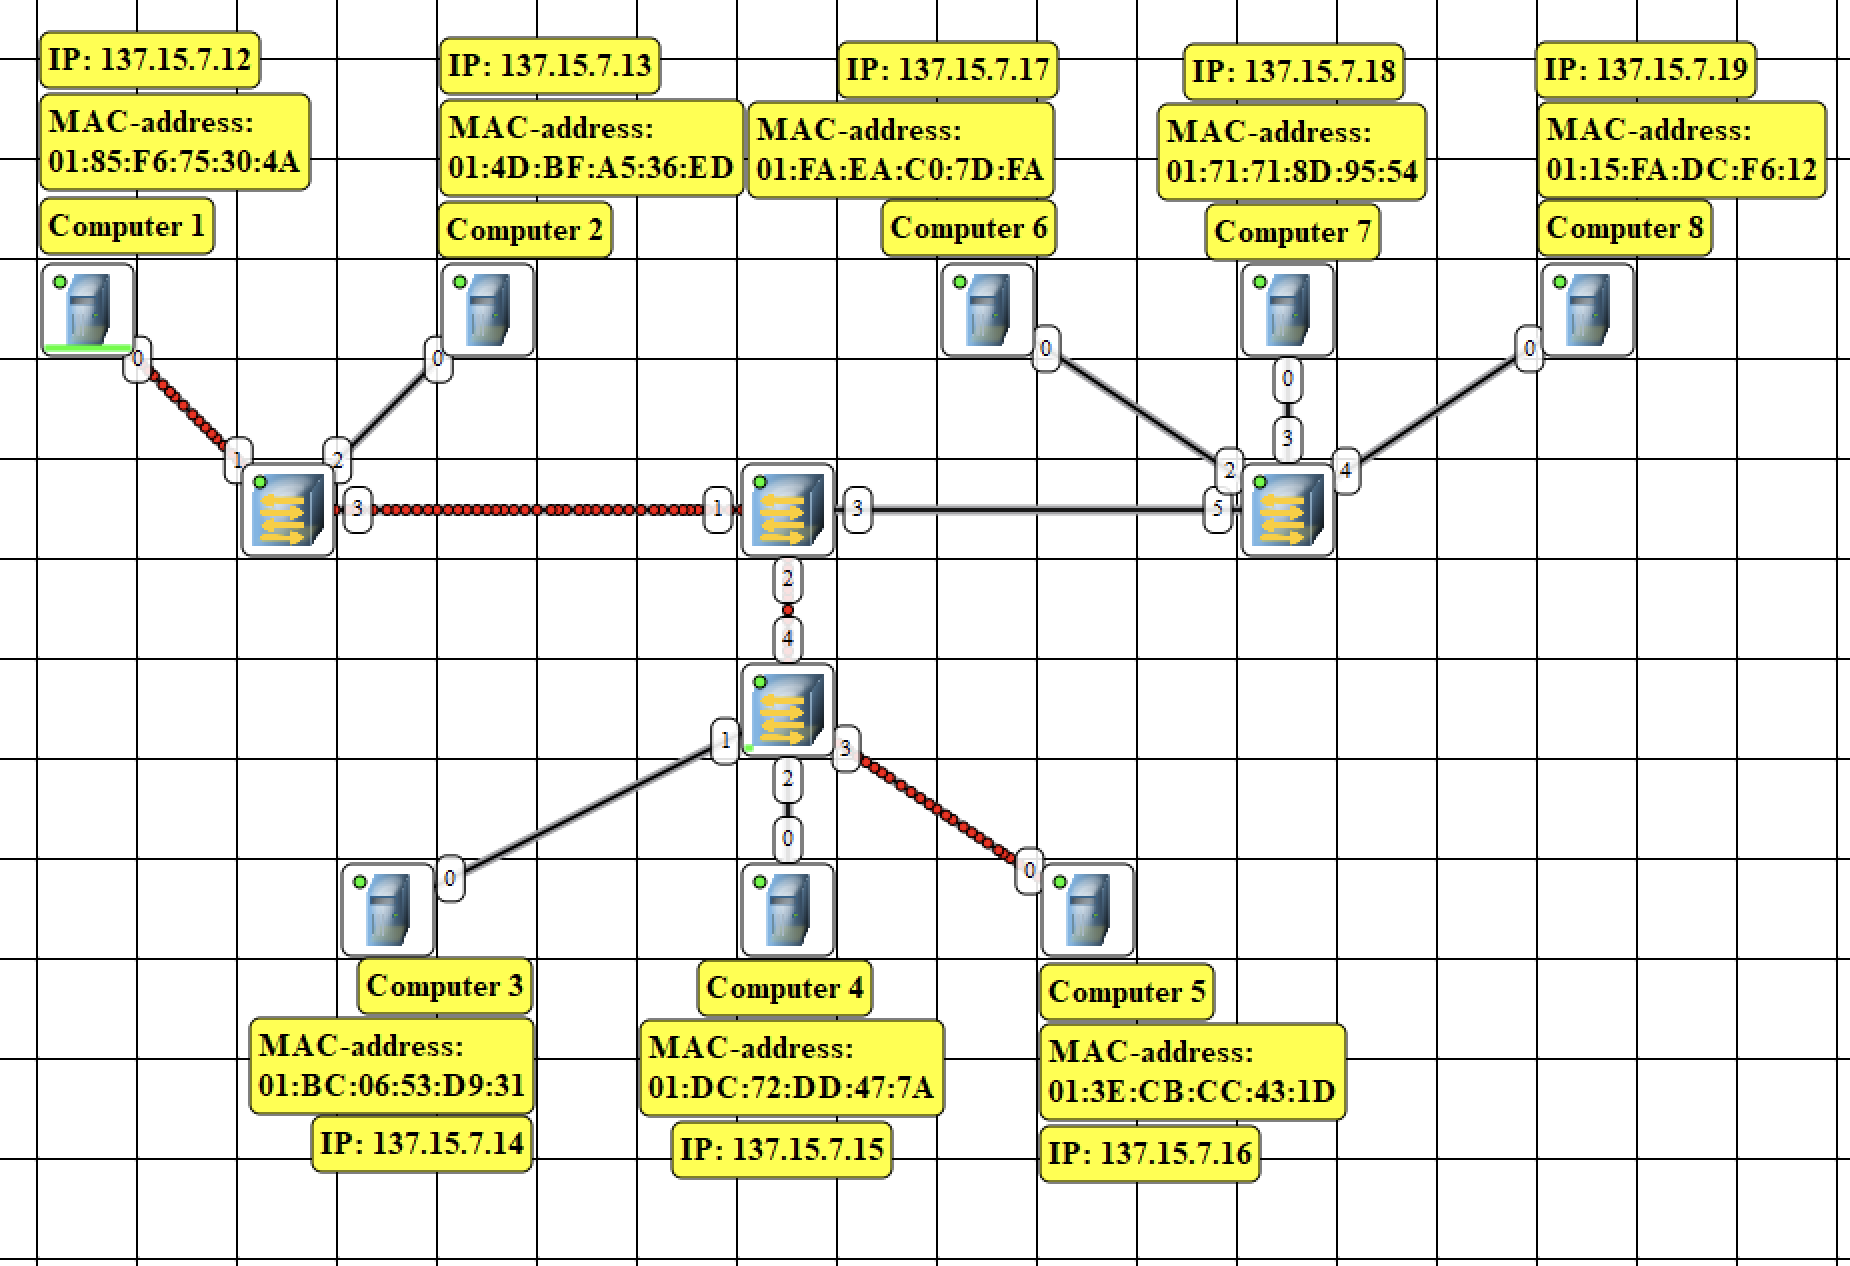
\includegraphics[width=\textwidth]{image/part3/udp-0.png}
  \caption{Отправка UDP-пакета с компьютера 1 на компьютер 5}
\end{figure}
\begin{figure}[H]
  \centering
  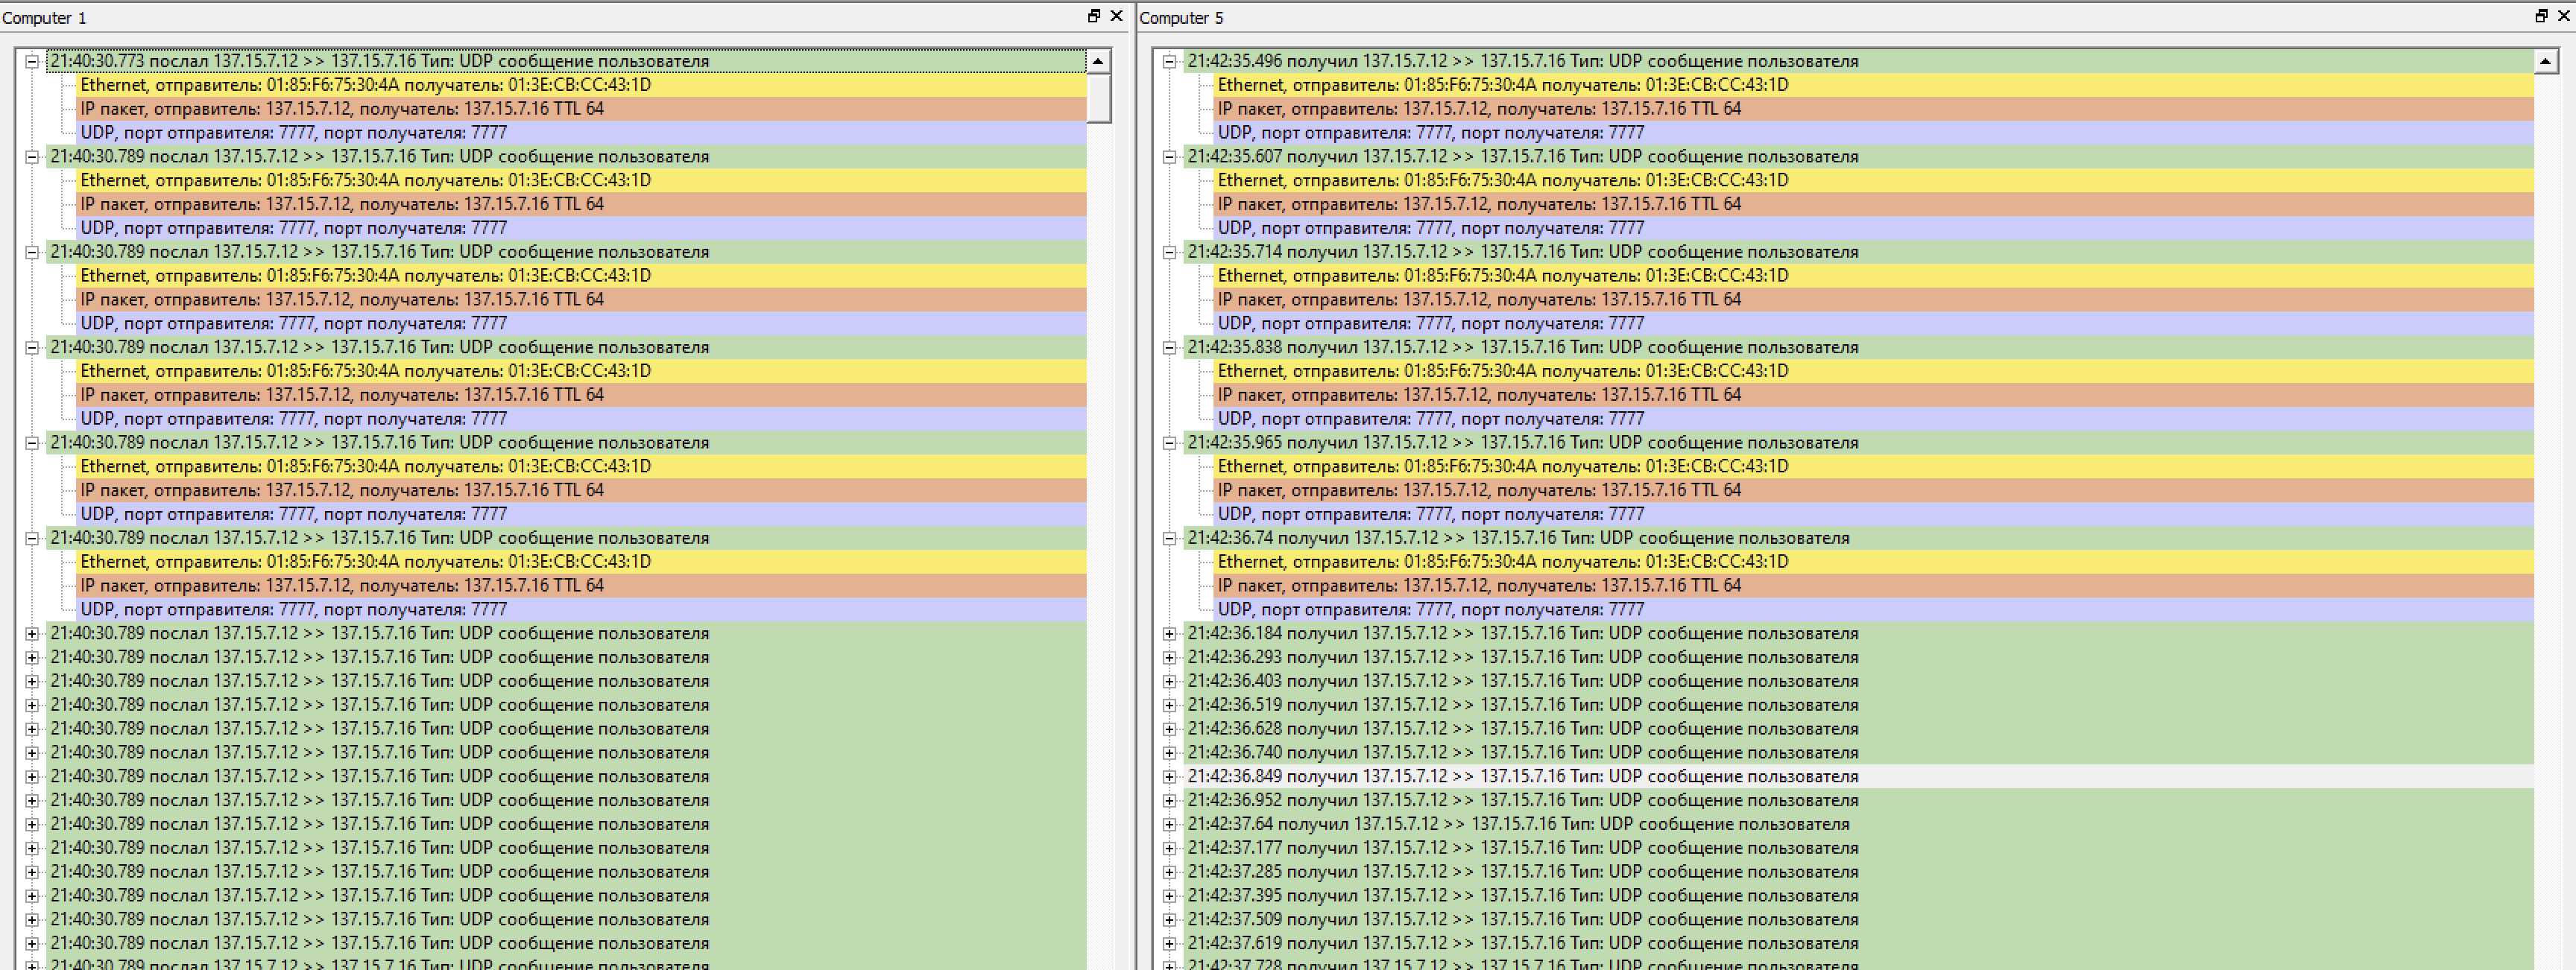
\includegraphics[width=\textwidth]{image/part3/udp-1.png}
  \caption{Отправка UDP-пакета с компьютера 1 на компьютер 5}
\end{figure}

Передача осуществляется по следующему алгоритму:
\begin{enumerate}
  \item Отправитель посылает ARP-запрос, который коммутаторами перенаправляется во все компьютеры и только итоговый получатель, посылает ответ
  \item Отправитель получает положительный ARP-ответ о наличии нужного компьютера в сети и посылает UDP-сообщение с данными
  \item Получателю доставлено UDP-сообщение
\end{enumerate}
Из-за того, что в нашей сети используются только коммутаторы, передача данных между любыми сегментами будет выглядеть аналогично тому, что было описано выше.

\subsection{TCP}
\begin{figure}[H]
  \centering
  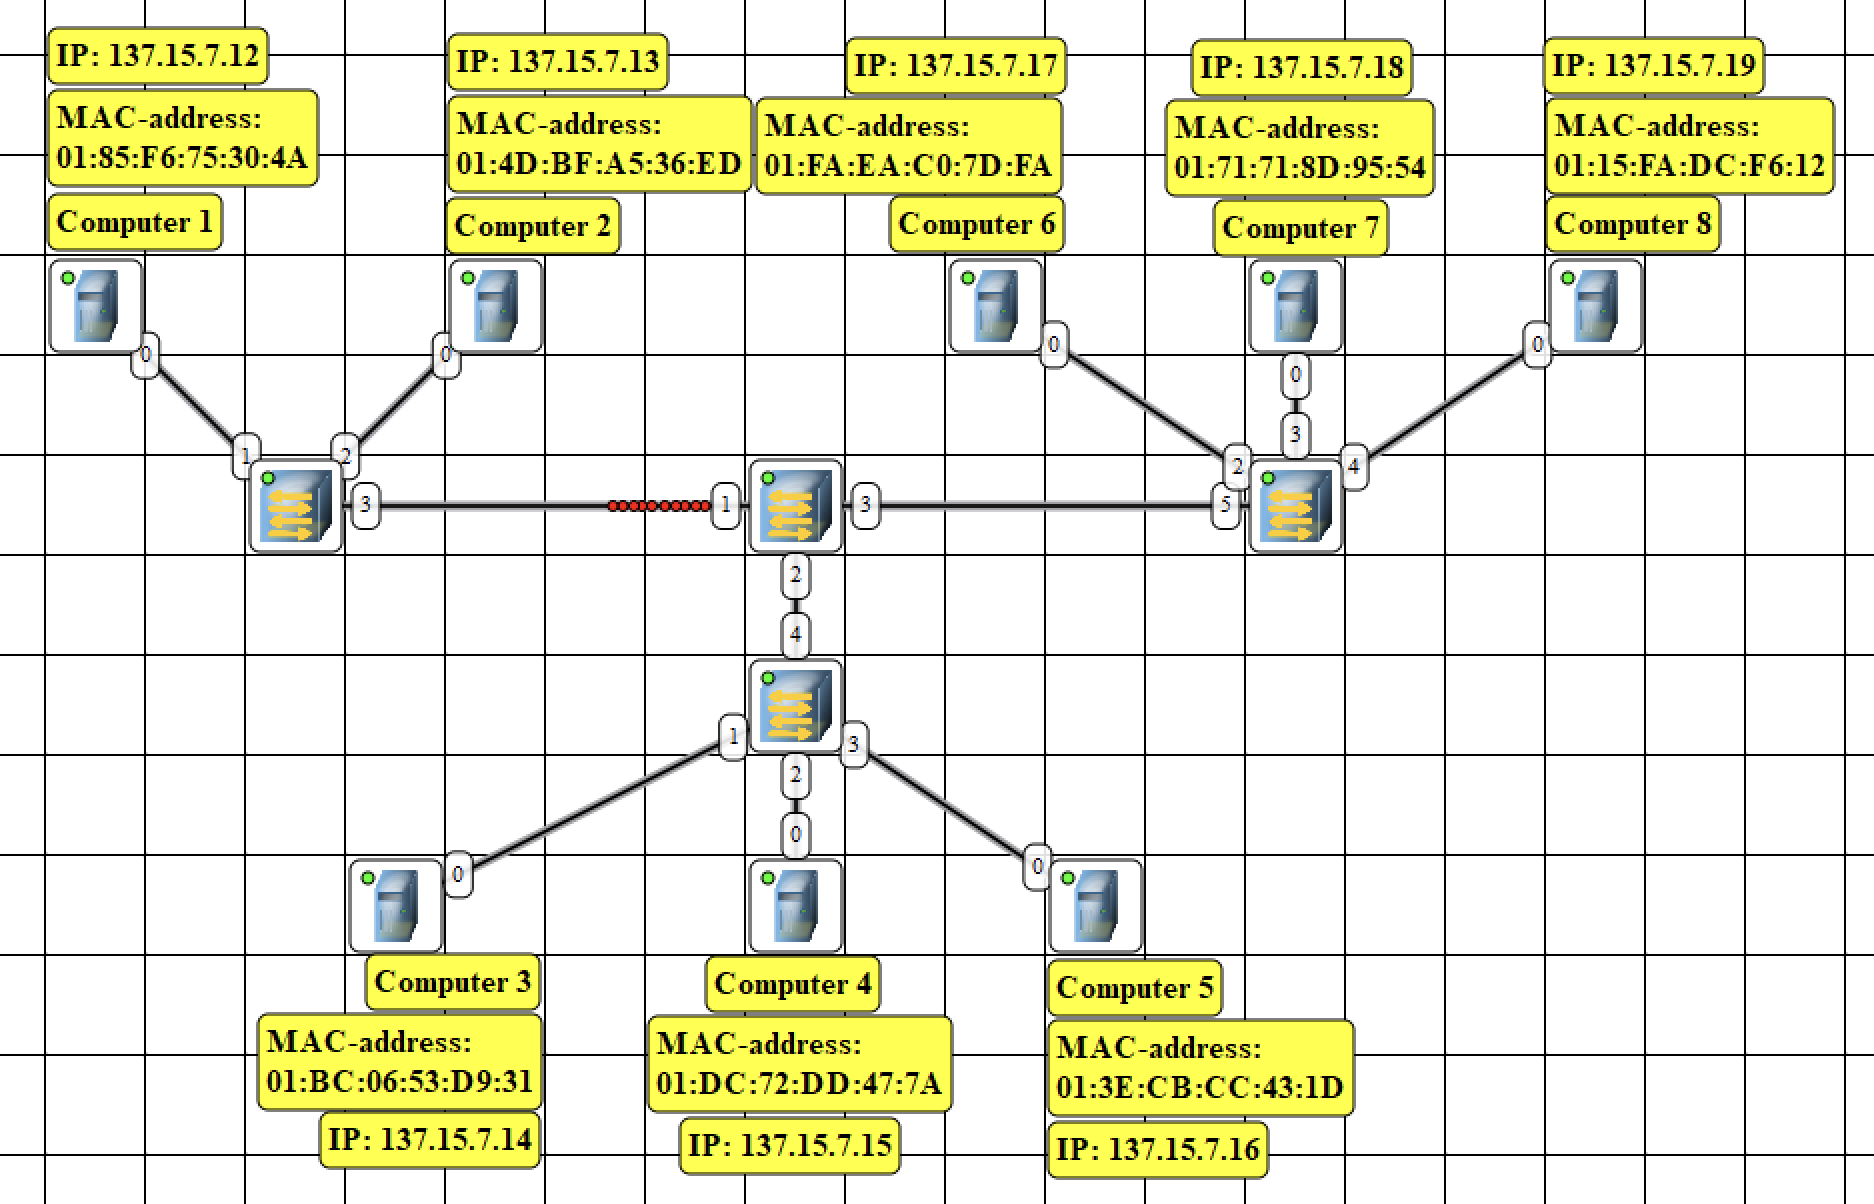
\includegraphics[width=\textwidth]{image/part3/tcp.png}
  \caption{Отправка TCP-пакета с компьютера 1 на компьютер 5}
\end{figure}
\begin{figure}[H]
  \centering
  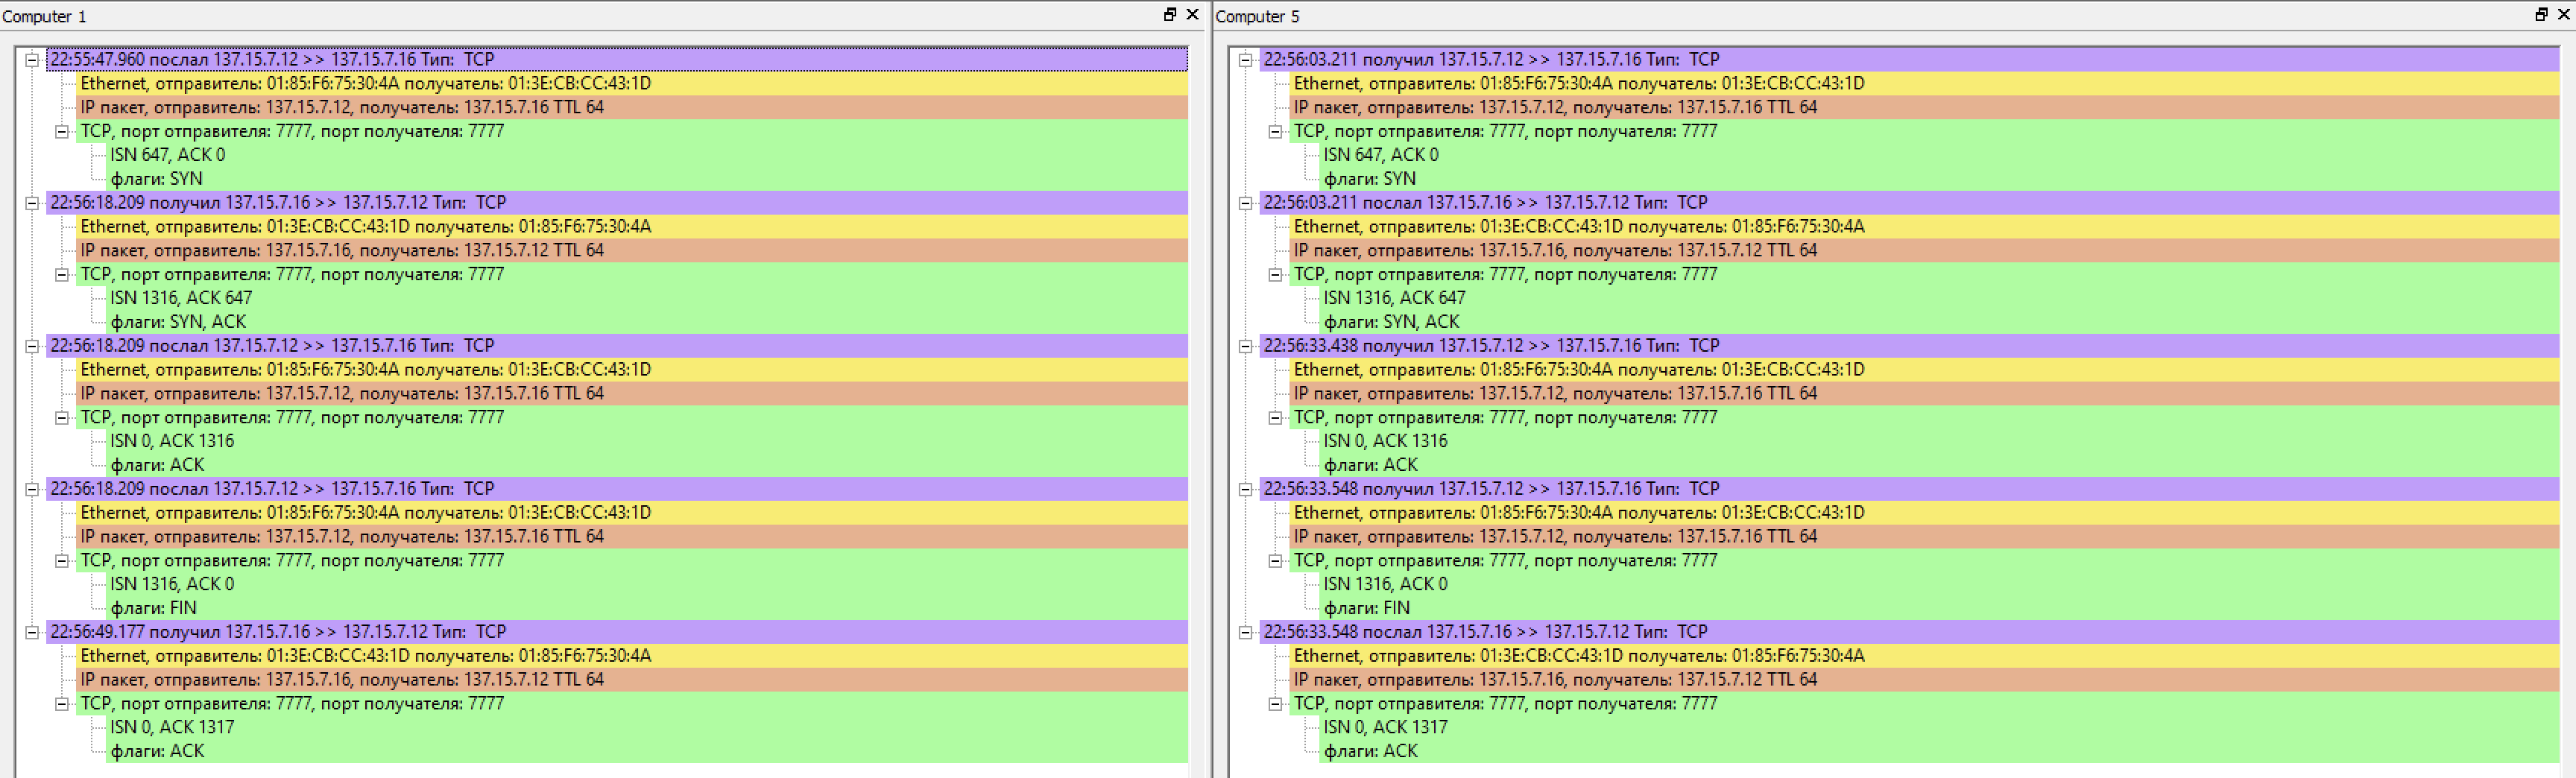
\includegraphics[width=\textwidth]{image/part3/tcp-1.png}
  \caption{Отправка TCP-пакета с компьютера 1 на компьютер 5}
\end{figure}

Передача осуществлялась по следующему алгоритму:
\begin{enumerate}
  \item Отправитель посылает TCP-запрос с флагом синхронизации и порядковым номером
  \item Получатель в ответ отправляет служебный TCP-запрос с флагами синхронизации и номером подтверждения
  \item Отправитель, посылает сообщение с номером подтверждение и второе сообщение с непосредственно данными и флагом окончания сообщения, поскольку объём передаваемых данных равен 1 килобайту и для этого хватит одного сообщения.
  \item Получатель, получив пакет с данными и флагом окончания сообщения, отправляет ответное сообщение с флагом номера подтверждения.
  \item Отправитель получает сообщение о том, что данные успешно получены и значит передача данных может быть завершена.
\end{enumerate}
Из-за того, что в нашей сети используются только коммутаторы, передача данных между любыми сегментами будет выглядеть аналогично тому, что было описано выше.
\section{Вывод}
В ходе выполнения лабораторной работы были изучены принципы настройки и функционирования локальных сетей, построенных с использованием концентраторов и коммутаторов, а также процессы передачи данных на основе стека протоколов TCP/IP и UDP, с использованием программы моделирования компьютерных сетей NetEmul.
Также была построена многосегментная локальная сеть, в которой были рассмотрены различные топологии сетей и их влияние на передачу данных.

\end{document}